\documentclass[12pt,a4paper,dvipsnames]{article}

\usepackage[T1]{fontenc}
\usepackage[utf8]{inputenc}
\usepackage[brazil]{babel}
\usepackage{amsmath,amsfonts,bezier,amstext,amsthm,amssymb}
\usepackage{geometry}
\usepackage{setspace}
\usepackage{comment}
\usepackage{graphicx}
\graphicspath{{figures/}}
\usepackage{multirow, bigstrut}
\usepackage{float}
\usepackage{hyperref}
\usepackage{subcaption}
\usepackage{tikz}
\usepackage{array}

\geometry{top=20mm,bottom=22mm,left=30mm,right=25mm}
\usetikzlibrary{shapes}

\newcommand{\PR}[1]{\ensuremath{\left[#1\right]}}
\newcommand{\PC}[1]{\ensuremath{\left(#1\right)}}
\newcommand{\BS}[1]{\ensuremath{\left|#1\right|}}
\newcommand{\BD}[1]{\ensuremath{\left\|#1\right\|}}
\newcommand{\chav}[1]{\ensuremath{\left\{#1\right\}}}
\newcommand{\tb}[1]{\ensuremath{\textbf{#1}}}
\newcommand{\mb}[1]{\ensuremath{\mathbf{#1}}}
\newcommand{\mc}[1]{\ensuremath{\mathcal{#1}}}
\newcommand{\Rn}[1]{\ensuremath{\mathbb{R}^{#1}}}
\newcommand{\In}[1]{\ensuremath{\mathbb{I}^{#1}}}
\newcommand{\hs}[1]{\hspace{#1}}

\newcommand{\secref}[1]{Seção~\ref{#1}}
\newcommand{\figref}[1]{Figura~\ref{#1}}
\newcommand{\eqnref}[1]{Equação~\eqref{#1}}
\newcommand{\tabref}[1]{Tabela~\ref{#1}}
\newcommand{\ssecref}[1]{Subseção~\ref{#1}}

\colorlet{MyRed}{OrangeRed!60!}
\newcommand{\improve}[1]{\textcolor{Green}{#1}}
\newcommand{\similar}[1]{\textcolor{MyRed}{#1}}

\setlength{\parskip}{1ex}
\setlength{\parindent}{1.1cm}

\tikzstyle{cred}=[circle, draw, thin,fill=red!80, scale=0.8]
\tikzstyle{cblue}=[circle, draw, thin,fill=cyan!80, scale=0.8]
\tikzstyle{iblue}=[circle, draw, thin,fill=cyan!100, scale=0.6]
\tikzstyle{cgreen}=[circle, draw, thin,fill=green!80, scale=0.8]
\tikzstyle{tgreen}=[circle, draw, thin,fill=green!80, scale=0.6]

\begin{document}

\thispagestyle{empty}

\begin{center}
{\LARGE Trabalho de Conclusão de Curso}
\vspace{0.5cm}

\begin{Large}\bf
Uma Implementação do Método FLIP para Simulação 2D de Fluidos
\end{Large}
\end{center}


\begin{center}
\begin{large}
Aluno: Gabriel Carvalho Sanches Rocha\\[0.5ex]
Orientador: Paulo Aristarco Pagliosa
\end{large}
\end{center}
\vspace{1cm}

\begin{abstract}
\noindent
Na área de computação gráfica, a animação baseada em física engloba simulações computacionais da dinâmica de corpos sólidos e/ou fluidos tal como são observados na natureza. Para a simulação de fluidos de forma numérica, podem ser utilizados solucionadores Lagrangianos, Eulerianos ou híbridos. Na abordagem Lagrangiana, ou material, a massa fluídica é discretizada em um sistema de partículas em que cada partícula representa uma parte da massa do fluido. Na abordagem Euleriana, ou espacial, emprega-se uma grade para discretizar a região que o fluido pode ocupar em células que armazenam informações do estado do fluido na região delimitada por essas células. Já os métodos híbridos, foco deste trabalho, combinam as abordagens Lagrangiana e Euleriana a fim de diminuir seus pontos negativos ao passo que aproveitam seus pontos positivos. Dentre os métodos híbridos, os estudados neste trabalho foram o \textit{particle-in-cell} (PIC) e o \textit{fluid-implicit-particle} (FLIP), ambos utilizando uma grade regular como método de subdivisão do espaço, isto é, usando células que têm as mesmas dimensões. O objetivo deste trabalho é apresentar uma implementação do método FLIP em C++ utilizando e estendendo a biblioteca CG desenvolvida durante a disciplina de Computação Gráfica. O resultado dessa implementação tem o propósito de servir como fundação em extensões futuras dos métodos híbridos, inicialmente para simulações bidimensionais, citando como exemplo o método FLIP com estruturas de subdivisão adaptativas tais como árvores quaternárias.
\end{abstract}

\section{Introdução}
\label{sec:introduction}

A animação baseada em física é amplamente empregada em diversas aplicações em ciências e engenharias, indústria de entretenimento e jogos digitais. Cada uma dessas aplicações tem objetivos diferentes e, portanto, valorizam um aspecto diferente. As aplicações para ciências e engenharias, por exemplo, requerem cálculos precisos para expressar e reproduzir fenômenos do mundo real que de outra maneira seriam mais difíceis e/ou custosos para simular. Já aplicações da indústria de entretenimento, especificamente as de efeitos especiais na cinematografia, têm ênfase na factibilidade visual, ou seja, o resultado produzido deve ser o mais indistinguível possível aos olhos humanos do esperado conforme a experiência cotidiana, assim tolerando-se maiores erros numéricos em comparação a aplicações para ciências e engenharias. Por fim, em aplicações para jogos digitais, em geral, a maior restrição é o processamento em tempo real. Isso implica sacrificar, em algum grau, precisão numérica e visual para obter resultados mais rápidos e proporcionar uma experiência fluida aos jogadores.

Para qualquer que seja a aplicação, as simulações utilizam de modelos para representar os corpos simulados. Desses modelos têm-se o geométrico --- uma representação exata ou aproximada da forma e dimensões de um objeto --- e o matemático, por meio da descrição do comportamento que governa esse corpo, geralmente descrito por equações diferenciais parciais e suas condições iniciais e de contorno. Tratando-se de modelos matemáticos, encontrar sua solução envolve o uso de um método numérico que forneça uma solução aproximada em uma versão discreta do objeto sendo simulado, isto é, através de partículas e/ou malhas de elementos de superfície e/ou volume.

O tipo de simulação mais comumente considerada em aplicações interativas é a de corpos rígidos. Um corpo rígido é um meio contínuo não deformável, isto é, a distância entre dois pontos do corpo é sempre a mesma, independente de qualquer esforço externo (forças e torques). A representação geométrica de um corpo rígido pode ser por composição de formas básicas (blocos, cápsulas e cilindros), malha de triângulos ou também um sistema de partículas, onde cada partícula concentra uma parcela da massa do corpo rígido. Já o comportamento de um corpo rígido é governado por uma equação de movimento derivada das leis de Newton, a qual relaciona grandezas como o estado do corpo (posição de seu centro de massa, orientação de seus eixos de inércia, velocidades linear e angular), sua inércia e esforços externos que nele atuam.

Outro tipo de simulação é a de sólidos deformáveis. Deformação é a transformação de um corpo de uma configuração de referência para a configuração corrente. Neste caso, configuração se refere ao conjunto de todas as posições das partículas do corpo ao longo do tempo. Um corpo deformável se classifica em elástico e plástico. O material de um corpo perfeitamente elástico é tal que recupera completamente sua configuração de repouso ao cessarem os esforços causadores da deformação. Em contraste, em um corpo plástico, parte das deformações são irreversíveis, mesmo retirados os esforços externos. Normalmente um material não é perfeitamente elástico, mas até certo limite, a partir do qual se comporta tal como um corpo plástico. Similar a um corpo rígido, um corpo deformável pode ser representado, geometricamente, por uma malha de polígonos ou sistema de partículas. Seu modelo matemático é dado por equações diferenciais derivadas da mecânica do contínuo \cite{malvern1969introduction}, as quais relacionam deslocamentos, deformações, tensões e forças de superfície e de volume aplicadas ao corpo. Para solucionar essas equações são empregados métodos numéricos, o mais amplamente empregado destes sendo o método dos elementos finitos (MEF) \cite{MEF}. O MEF submete o corpo a uma discretização em nuvem de pontos, também conhecidos por nós ou pontos nodais, interligados por meio de elementos chamados elementos finitos, por exemplo, tetraedros no caso tridimensional. Como resultado da discretização, encontra-se uma solução aproximada para um sistema de equações algébricas cuja solução fornece os deslocamentos (por consequência, as deformações) em cada ponto nodal. Para obter os deslocamentos em pontos internos de um elemento finito, usa-se interpolação dos deslocamentos dos nós nos quais o elemento incide, considerandos os pesos definidos pela chamada função de forma do elemento.

De maneira similar aos corpos rígidos e deformáveis, emprega-se a simulação de fluidos em aplicações das mais diversas finalidades. Um fluido é um meio contínuo que oferece pouca resistência a esforços cortantes. Isso significa que esse corpo sofre deformação continuamente à medida que é submetido a forças, a exemplo da água ou fumaça. Assim como corpos rígidos e deformáveis, a geometria dos fluidos pode ser representada por malhas de polígonos ou por um sistema de partículas. O comportamento dos fluidos é modelado por equações diferenciais derivadas da mecânica do contínuo. Assim, fluidos incompressíveis são modelados pelas equações de Navier-Stokes, apresentadas na \secref{sec:flipmethod}, porém, os fatores dominantes da simulação são diferentes de acordo com a escala observada, a exemplo dos gases da atmosfera ou gotículas de água. Dito isso, este trabalho considera, por simplicidade, apenas fluidos que são líquidos incompressíveis, ou seja, que não variam em volume quando submetidos a esforços, como são os líquidos mais comuns observados no dia-a-dia.

Existem três abordagens para a solução numérica das equações de Navier-Stokes: Lagrangiana, Euleriana e híbrida. Na abordagem Lagrangiana, ou material, acompanhamos o fluido por um sistema de partículas no qual cada partícula representa uma parcela da massa fluídica. Às partículas associam-se quatro grandezas: posição, velocidade, pressão e força externa. Com essa modelagem, para simular o fluido é necessário determinar, a cada passo de tempo ao longo da simulação, a posição e a velocidade para cada partícula do fluido, em termos das forças que atuam sobre cada uma. Um exemplo de método Lagrangiano é o \textit{smoothed particle hydrodynamics} (SPH) \cite{SPH, egst.20141034}. Quanto à abordagem Euleriana, ou espacial, usa-se um método de subdivisão do espaço de simulação em células, as quais armazenam grandezas do fluido que passa por elas. Desta forma, atualizam-se as parcelas de fluido nas células de acordo com as grandezas contidas na grade, a cada passo de tempo.

Nas abordagens híbridas, principal foco deste trabalho, as abordagens Lagrangiana e Euleriana são mescladas com intuito de compensar suas desvantagens particulares e agregar seus pontos positivos. Um exemplo de método híbrido é o \textit{particle-in-cell} (PIC) \cite{PIC}, que acompanha o fluido de forma Lagrangiana, usando partículas e realizando os cálculos das forças que movimentam o fluido na grade. Como extensão do método PIC, há outro método híbrido chamado \textit{fluid-implicit-particle} (FLIP) \cite{FLIP, NarrowBandFlip, extendedNarrowBandFlip}, que diminui a introdução de viscosidade artificial oriunda do PIC. Os modelos híbridos são tratados na \secref{sec:flipmethod}. De acordo com o exposto acima, os objetivos específicos do trabalho são:
\begin{itemize}
\item[\tb{O1}] Estudar os métodos híbridos PIC e FLIP; e

\item[\tb{O2}] Implementar o PIC e FLIP para simulação de fluidos em duas dimensões.

\end{itemize}

Como principal contribuição, tem-se que a implementação servirá de base para implementação, e também como modelo de comparação, para uma extensão dos métodos híbridos utilizando grades adaptativas como alternativas às grades regulares empregadas neste trabalho. Esta extensão é o foco de um projeto de mestrado em andamento. A motivação para essa abordagem se dá pois, com uso de grades regulares, é possível que se tenha um problema de distribuição irregular do volume do fluido, isto é, pode haver muito espaço com pouco ou nenhum fluido e uma concentração alta de fluido em espaços menores. Essa irregularidade não é tratada pela grade regular, que processa todas as células independente de conter fluido ou não, e se intensifica à medida que a granularidade da grade diminui, com impactos no tempo de processamento. Para lidar com este problema proveniente das grades regulares, no referido projeto propõe-se o uso de grades adaptativas, as quais subdividem o espaço de acordo com a concentração de fluido, ou seja, mais células onde a concentração do fluido é alta e menos onde é baixa (ou nenhuma), sendo as árvores quaternária (\textit{quadtree}) e octária (\textit{octree}) as estruturas mais comuns em ambientes bidimensionais e tridimensionais, respectivamente.

O restante do texto é organizado como segue. A \secref{sec:flipmethod} é dedicada ao método FLIP, que dá título a este trabalho, além de apresentar as equações que modelam o comportamento dos fluidos incompressíveis, as equações de Navier-Stokes, e outros conceitos importantes para o entendimento de simulações de fluidos. A \secref{sec:implementation} apresenta a abordagem prática tomada para o desenvolvimento do solucionador FLIP, implementado com o uso de grade regular. A \secref{sec:results} apresenta o resultado de quatro simulações utilizando o solucionador implementado, bem como as parametrizações utilizadas. Por fim, a \secref{sec:conclusion} conclui o trabalho e apresenta possíveis extensões e trabalhos futuros.

\section{O método FLIP}
\label{sec:flipmethod}

% Fazer subseção para fundamentos
% Trocar Eq. Governantes por outro termo

\subsection{Fundamentos}
\label{ssec:fundamentals}

Conforme mencionado, os fluidos são meios contínuos que oferecem pouca resistência a esforços cortantes e incluem líquidos e gases. Os líquidos tomam a forma do recipiente que os contém enquanto os gases expandem ao máximo quando não contidos. Os fluidos se classificam em compressíveis e incompressíveis, sendo compressíveis os que podem variar em volume quando submetidos a forças externas e \textit{incompressíveis} o exato oposto, resistindo à compressão independente da sua intensidade. O restante do conteúdo desta seção é baseado no Capítulo 1 de \cite{kim_2017}.

Dentre as propriedades dos fluidos, podemos destacar: velocidade, densidade, pressão e viscosidade. A velocidade relaciona uma quantia de tempo com o deslocamento do fluido no espaço. A pressão é a relação entre uma força e sua área de atuação e a densidade é a razão entre a massa de um fluido e seu volume, podendo variar com mudanças na velocidade ou pressão. Enfim, a viscosidade é a propriedade do fluido que caracteriza sua resistência a esforços cortantes, sendo que quanto mais viscoso um fluido mais ``pastoso'' este é.

\paragraph{Equações de Navier-Stokes.} As propriedades dos fluidos incompressíveis são modeladas pelas Equações de Navier-Stokes \cite{malvern1969introduction}, as quais são expressas com o uso de operadores diferenciais da seguinte forma:
% Estas propriedades se traduzem matematicamente nas equações de Navier-Stokes, as quais modelam o comportamento de fluidos incompressíveis. Estas encontram-se abaixo expressas com uso de operadores diferenciais:
\begin{align}
    \frac{\partial \Vec{u}}{\partial t} + \Vec{u} \cdot \nabla \Vec{u} + \frac{\nabla p}{\rho} & = \Vec{g} + \mu \nabla^2 \Vec{u}, \label{eq:momentum}\\
    \nabla \cdot \Vec{u} & = 0, \label{eq:pressure}
\end{align}
em que $\Vec{u}$ representa a velocidade do fluido e $\Vec{g}$ representa a aceleração da gravidade. O tempo é denotado por $t$ e a pressão por $p$. As letras gregas $\rho$ e $\mu$ denotam a densidade e viscosidade do fluido, respectivamente. Para o entendimento completo das equações de Navier-Stokes, é necessário definir também os operadores diferenciais empregados. O operador \textit{gradiente}, denotado por $\nabla$, para uma função escalar $f: \mathbb{R}^n \to \mathbb{R}$, é dado por:
%
\begin{equation}
    \nabla f = \left(\frac{\partial f}{\partial x_1}, \frac{\partial f}{\partial x_2}, \cdots, \frac{\partial f}{\partial x_n} \right).
\end{equation}
O resultado deste operador é um vetor que aponta para a direção de maior variação do campo escalar dado pela função. Já quando aplicado a uma função vetorial, o gradiente tem a forma de uma matriz Jacobiana. Tendo-se uma função vetorial $\Vec{f}: \mathbb{R}^n \to \mathbb{R}^m$ é possível interpretar cada coordenada desta função como uma função escalar $f_i$, para $1 \leq i \leq m$, desta maneira, o gradiente é definido por:
%
\begin{equation}
    \nabla \Vec{f} =
    \begin{bmatrix}
    \frac{\partial f_1}{\partial x_1}  & \cdots & \frac{\partial f_1}{\partial x_n} \\
    \vdots & \ddots & \vdots \\
    \frac{\partial f_m}{\partial x_1}  & \cdots & \frac{\partial f_m}{\partial x_n} \\
    \end{bmatrix}.
\end{equation}
Além do gradiente, na \eqnref{eq:pressure} usa-se o operador \textit{divergente}, denotado por $\nabla \cdot$. De modo geral, este operador transforma um campo vetorial em um campo escalar que  mede o fluxo de entrada e saída do campo original em um volume infinitesimal. Formalmente, tem-se para uma função vetorial $\Vec{f}: \mathbb{R}^m \to \mathbb{R}^m$:
%
\begin{equation}
    \nabla \cdot \Vec{f} = \sum_{i = 1}^{m} \frac{\partial f_i}{\partial x_i}.
\end{equation}
Por fim, tem-se o operador de Laplace, denotado por $\nabla^2$, que é o resultado do operador divergente aplicado ao gradiente de um campo escalar. De maneira informal, este operador representa os ``solavancos'' de um campo. Para uma função escalar $f: \mathbb{R}^n \to \mathbb{R}$ este operador é dado por:
\begin{equation}
    \nabla^2 f = \nabla \cdot \nabla f = \sum_{i = 1}^{n} \frac{\partial^2 f}{\partial x_i^2}.
\end{equation}
Para o uso do operador Laplaciano em campos vetoriais, toma-se uma abordagem similar a do gradiente, na qual avalia-se o Laplaciano para cada função $f_i$ como segue:
%
\begin{equation}
    \nabla^2 \Vec{f} = (\nabla^2 f_1, \nabla^2 f_2, \cdots, \nabla^2 f_m).
\end{equation}

A primeira das equações de Navier-Stokes, \eqnref{eq:momentum}, é chamada de equação de momento, isto é, a Segunda lei de Newton adaptada para fluidos incompressíveis. Nela, tem-se que a diferença entre as forças externas e internas atuando sobre o fluido é igual ao produto entre a massa e a aceleração. Analisando a \eqnref{eq:momentum} por termos auxilia no entendimento de como cada propriedade de um fluido se apresenta:
\begin{align}
\label{eq:momentum2}
    \overbrace{\frac{\partial \Vec{u}}{\partial t} + \Vec{u} \cdot \nabla \Vec{u}}^{a} + \overbrace{\frac{\nabla p}{\rho}}^{b} & = \Vec{g} + \overbrace{\mu \nabla^2 \Vec{u}}^{c},
\end{align}
Na \eqnref{eq:momentum2}, o termo $(a)$ é chamado de derivada material, representando a taxa de variação de uma grandeza ao longo do tempo para uma parcela de fluido movendo-se a uma velocidade $\Vec{u}$. O termo $(b)$ é a razão que mede a força da pressão de uma parcela de fluido. Por fim, o termo $(c)$ do lado direito da equação representa a força viscosa, a qual tenta diminuir a diferença de velocidade de uma partícula em relação a suas vizinhas. A \eqnref{eq:pressure} é a condição de incompressibilidade e garante que o fluido é incompressível ao restringir o divergente da velocidade a zero, isto é, garante que não existe fluxo para dentro ou para fora de nenhuma parcela de fluido. Para que a solução das equações diferenciais seja única, é necessária a adoção de condições de contorno, isto é, restrições associadas às equações para definir como solucioná-las na borda do domínio. Para as equações de Navier-Stokes, essas condições de contorno são responsáveis por restringir o fluxo nas bordas de sólidos. Comumente, usam-se as condições de contorno de Dirichlet --- a qual restringe os valores de uma função, por exemplo, a velocidade, em pontos do contorno do fluido --- e de Newmann, que restringe os valores da derivada direcional de uma função, por exemplo, fluxo, na direção das normais do contorno. Maiores detalhes podem ser obtidos em \cite{kim_2017, bridson_2016}.

Além das equações de momento e de incompressibilidade, o movimento do fluido também é limitado nas interfaces com sólidos, aos quais chamam-se colisores. Tais limitações são dadas pela aplicação das \textit{condições de contorno} de Newmann e Dirichlet no campo velocidade, gerando as condições \textit{no-flux} e \textit{free/no-slip} respectivamente. A condição \textit{no-flux} impede a penetração de fluido em bordas sólidas enquanto \textit{free-slip} e \textit{no-slip} permite e restringe respectivamente, o movimento do fluido em direções tangentes à borda. Matematicamente, a condição de borda \textit{no-flux} é escrita por:
%
\begin{equation}
    \Vec{u} \cdot \Vec{n} = 0,
    \label{eq:noflux}
\end{equation}
ou seja, a velocidade $\Vec{u}$ do fluido em bordas sólidas deve ser perpendicular à normal da superfície, representada por $\Vec{n}$. Para as condições \textit{slip} usa-se um meio termo entre restringir totalmente (\textit{no-slip}) e não restringir (\textit{free-slip}) o movimento nas bordas, de acordo com:
%
\begin{equation}
    \label{eq:slipcond}
    \Vec{u} = \text{max}\left( 1 - \lambda \frac{\text{max}\left(-\Vec{u} \cdot \Vec{n},0\right)}{\lvert \Vec{u}_{p}\rvert}, 0\right) \Vec{u}_{p},
\end{equation}
em que $\lambda$ é o coeficiente de fricção da superfície, que restringe a velocidade, e $\Vec{u}_p$ é a velocidade projetada na superfície.

Para simular efetivamente um fluido, os métodos Lagrangianos, Eulerianos e híbridos devem solucionar as equações de Navier-Stokes. Para tanto, calculam e então acumulam forças externas, incluindo gravidade e forças de arrasto (forças que se opõem ao movimento de um sólido em meio a um fluido), força viscosa e pressão. Para o cálculo da força viscosa aplica-se o operador Laplaciano no campo de velocidade. Por fim, o cálculo da pressão é feito calculando a densidade e então aplicando seu gradiente. Além desses passos, nos métodos baseados em grade é necessário um passo de advecção, que é a transferência de matéria ao longo do fluxo do fluido. Apesar de solucionarem as mesmas equações, a maneira que cada método o faz é diferente em decorrência da própria modelagem subjacente, com os métodos Lagrangianos usando partículas e métodos Eulerianos usando uma grade. Como consequência, a maneira de calcular as Equações \eqref{eq:momentum} e \eqref{eq:pressure} é diferente entre essas abordagens.

Como o cômputo das referidas equações de Navier-Stokes envolve determinar operadores diferenciais, no caso das abordagens Eulerianas e híbridas, tal como PIC e FLIP, comumente usa-se o método das \textit{diferenças finitas} \cite{levequeFDM} para obter uma aproximação desses operadores. Nas grades regulares, a informação pode ser armazenada em diferentes pontos de uma célula, como seu centro, ou o centro de suas faces. Com isso, o uso das diferenças finitas relaciona a célula que contém o ponto no qual deseja-se avaliar o operador e pontos nas células vizinhas. A configuração que esses pontos formam se chama \textit{stencil}, conforme o exemplo na \figref{fig:stencil}.

\begin{figure}[ht]
    \centering
    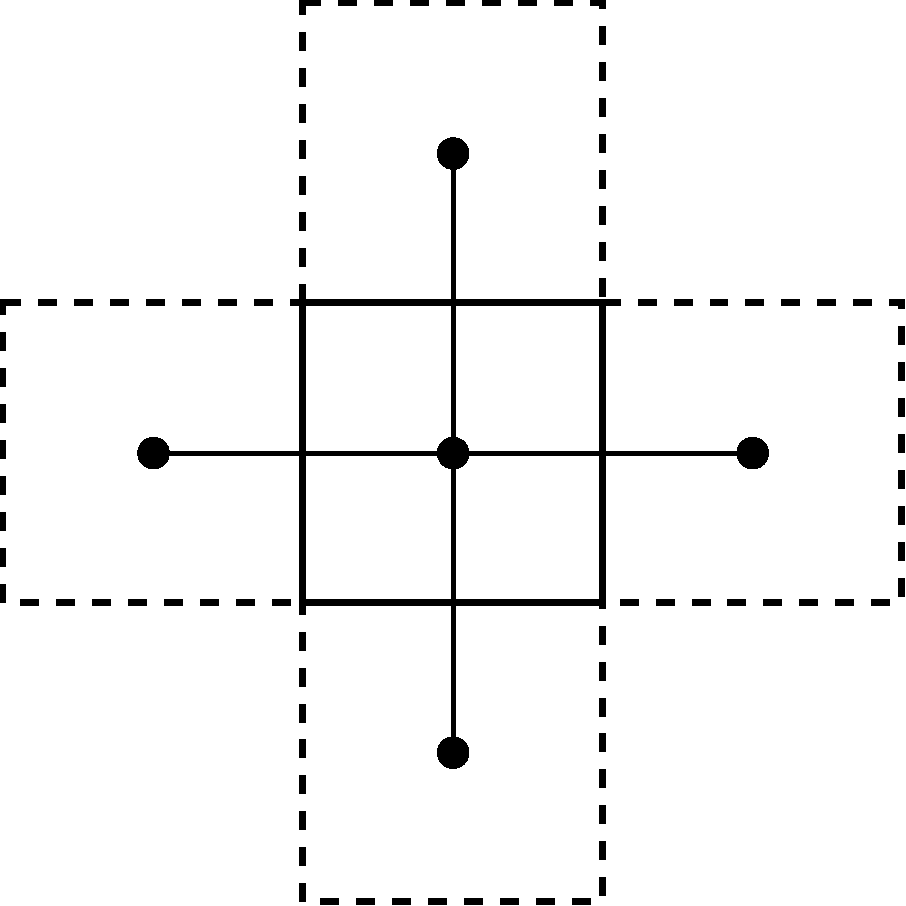
\includegraphics[width=0.3\textwidth]{Stencil.pdf}
    \caption{\textit{Stencil} em uma grade regular com pontos de controle nos centros das células.}
    \label{fig:stencil}
\end{figure}

Em grades regulares, os \textit{stencils} associados ao centro de uma célula possuem configuração exatamente como apresentada na \figref{fig:stencil}. Como consequência, é possível avaliar a derivada parcial, fundamental para o cálculo de todos os operadores diferenciais, em função dos valores da função desejada nos pontos do \textit{stencil}, e com isso computar os diferentes operadores. Seja $f(x, y)$ uma função avaliada para todos os pontos de uma célula $(i, j)$ de uma grade regular bidimensional com espaçamento $(\Delta x,\Delta y)$. A derivada parcial de $f$ em relação a $x$ é dada por:
\begin{equation}
    \frac{\partial f}{\partial x} \approx \frac{f^{i+1, j} - f^{i,j}}{\Delta x}.
\end{equation}
Esta equação é conhecida como diferença finita progressiva, por medir a derivada parcial na direção positiva do eixo adotado. Além desta, existem as diferenças finitas regressiva e central, sendo a última uma média entre a progressiva e regressiva, dada por:
\begin{equation}
    \frac{\partial f}{\partial x} \approx \frac{f^{i+1, j} - f^{i-1,j}}{2\Delta x}.
\end{equation}
Esta será utilizada para ilustrar o cálculo dos operadores diferenciais. Nota-se que a qualidade da aproximação usando diferenças finitas está diretamente ligada ao espaçamento, de forma que quanto menor o espaçamento da grade melhor a aproximação.

A partir das diferenças finitas para aproximar as derivadas parciais, torna-se possível calcular os operadores diferenciais. Aplicando-se a diferença finita central para aproximar as derivadas parciais no cálculo do gradiente, tem-se:
\begin{equation}
    \nabla f(x) \approx \left( \frac{f^{i+1, j} - f^{i-1,j}}{2\Delta x}, \frac{f^{i, j+1} - f^{i,j-1}}{2\Delta y} \right).
\end{equation}
Com a mesma ideia é possível definir os outros operadores, tomando como outro exemplo o operador divergente:
\begin{equation}
    \nabla \cdot f(x) \approx \frac{f^{i+1, j} - f^{i-1,j}}{2\Delta x} +  \frac{f^{i, j+1} - f^{i,j-1}}{2\Delta y}.
\end{equation}

\subsection{Métodos híbridos PIC e FLIP}
\label{ssec:hibridmethods}

% [TODO] Adicionar Imagem mostrando as particulas e mostrando as grades

No que tange os pontos positivos e negativos das abordagens Lagrangiana e Euleriana, acerca do método material tem-se boa conservação de grandezas físicas associadas às partículas, como massa e momento e, além disso, este trata sem complicações a interação do fluido com outros corpos na simulação. Em contrapartida, o método Lagrangiano não admite passos de tempo muito grandes e também pode, em decorrência da distribuição das partículas, introduzir ruídos na simulação. Quanto aos métodos Eulerianos, têm-se resultados mais suaves e possibilidade de usar passos de tempo maiores. Entretanto, viscosidade artificial é introduzida por conta da dissipação numérica advinda das transferências na advecção. Por fim, os métodos híbridos usam os dois métodos para atenuar seus problemas.

O primeiro método híbrido estudado foi o PIC (\emph{particle in cell}). Este discretiza o espaço de simulação com uso de uma grade regular, tal como um método espacial, mas acompanha o fluido usando partículas, a fim de se atenuar o problema de dissipação numérica na advecção. No PIC, usam-se partículas para indicar quais células da grade possuem fluido, enquanto todas as propriedades e interações do fluido, como colisões, são calculadas com o uso da grade. Em um passo de tempo $\Delta t$ da simulação, os passos do PIC essencialmente são:
\begin{itemize}
    \item [\tb{P1}] Transferir velocidade das partículas para grade;
    \item [\tb{P2}] Calcular forças externas, viscosidade e pressão;
    \item [\tb{P3}] Transferir velocidade da grade para as partículas; e
    \item [\tb{P4}] Mover cada partícula com sua nova velocidade.
\end{itemize}

Para transferir a velocidade das partículas para a grade, é feita uma distribuição da mesma para os pontos da grade mais próximos da partícula. Essa distribuição usa as coordenadas baricêntricas da partícula em relação à célula da grade na qual a partícula está contida, tomando-se os vértices da célula como pontos de controle. Em outras palavras, como visto na \figref{fig:transferparticlecell}, a velocidade $\Vec{u}$ de uma partícula é dividida proporcionalmente entre os pontos de controle da célula que a contém de acordo com as subáreas formadas quando traçadas linhas horizontal e vertical paralelas aos eixos da grade. Esta distribuição é repetida para cada partícula e, por fim, a velocidade resultante em cada ponto da grade é a média ponderada das velocidades transferidas. É importante ressaltar que os passos de transferência entre partículas e grade, e vice e versa, são independentes do tipo de grade adotado, podendo ser como no exemplo, uma grade com pontos de controle nos cantos da célula ou com pontos de controle nas faces da célula, como adotado na implementação, abordada na \secref{sec:implementation}.

\begin{figure}[ht]
\centering
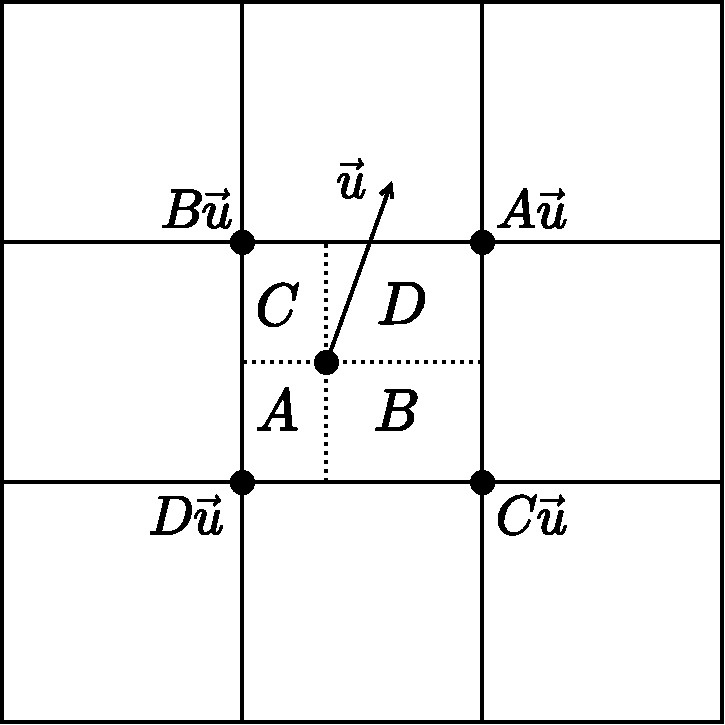
\includegraphics[width=0.35\textwidth]{Particle2Grid.pdf}
\caption{A velocidade é distribuída para os pontos da grade de acordo com as coordenadas baricêntricas da partícula em relação à célula que a contém, como pode ser observado geometricamente pelas subáreas $A$, $B$, $C$ e $D$. Adaptado de \cite{kim_2017}.}
\label{fig:transferparticlecell}
\end{figure}

Após o primeiro passo de transferência, calculam-se forças externas, viscosidade e pressão como no método Euleriano. Dessas grandezas, as forças externas e viscosidade são armazenadas nos centros das faces das células, assim como a velocidade, enquanto a pressão é associada aos centros das células, para que ao calcular o seu gradiente, este seja acumulado também aos centros das faces. Para as forças externas, originalmente apenas a gravidade, somam-se as componentes de $\Delta t \Vec{g}$ diferentes de zero ao campo velocidade. Em seguida, calcula-se a viscosidade --- que como dito anteriormente, procura diminuir a diferença de velocidade de um ponto em relação aos seus vizinhos --- usando o método de Euler , seja explícito ou implícito, para solucionar $\mu\nabla^2\Vec{u}$, o termo $c$ da \eqnref{eq:momentum2}. Os método de Euler proveem aproximações numéricas para equações diferenciais dependentes de tempo, de forma que o método explícito calcula a solução para o tempo posterior usando a solução para o tempo atual, enquanto o método implícito encontra a solução associando ambas soluções, mais detalhes encontram-se em \cite{kim_2017}. À primeira vista, usar o método de Euler explícito parece mais atrativo por eficiência computacional, porém a estabilidade dos resultados com seu uso depende da viscosidade do fluido estar abaixo de um limiar bastante restrito, mais detalhes sobre esse limiar encontram-se em \cite{kim_2017}. Com isso, apesar do maior custo computacional, a opção mais robusta, que garante estabilidade para fluidos mais viscosos e suporta passos de tempo maiores, é o método de Euler implícito. Por fim, usa-se a mesma ideia para o cálculo da pressão e posteriormente seu gradiente, dado por $\frac{\nabla p}{\rho}$ conforme item $b$ da \eqnref{eq:momentum2}.

A transferência das velocidades (dos pontos dos cantos das células) da grade para as partículas é realizada por meio de interpolação bilinear, para o caso bidimensional. Da mesma maneira que foram usadas as coordenadas baricêntricas para transferência de partícula para grade, as células transferem suas velocidades para as partículas nela contidas. Por fim, atualizadas as velocidades de cada partícula resta movê-las, isso é feito pela regra do ponto médio, como segue:
\begin{itemize}
    \item [\tb{P1}] Obtém-se o ponto médio deslocando a partícula com sua velocidade por metade do passo de tempo;
    \item [\tb{P2}] Interpola-se a velocidade para a o ponto médio;
    \item [\tb{P3}] A partícula é deslocada com a velocidade interpolada pelo passo de tempo completo.
\end{itemize}
  
Apesar dos benefícios do método PIC em comparação com métodos exclusivamente Eulerianos, como por exemplo a conservação da massa pelo uso das partículas, esse ainda sofre de problemas de dissipação numérica provenientes, agora, não da advecção mas das sucessivas transferências entre partículas e grade. Novamente, este problema introduz viscosidade artificial ao fluido. Para contornar esse problema, o método flip (\emph{fluid-implicit-particle}) pode ser utilizado.

O FLIP é uma extensão do método PIC proposta por Brackbill e Ruppel \cite{FLIP} em que, com mudanças mínimas, obtém-se redução na dissipação numérica. O método soluciona este problema por interpolar, no passo de transferência da grade para as partículas, a diferença entre as velocidades final --- produto das forças internas e externas --- e inicial --- obtida após a transferência das partículas para a grade --- e somá-la à velocidade da partícula. A \figref{fig:transfercellparticle} ilustra o método de transferência proposto, em que $\Delta$ denota a diferença entre as velocidades final e inicial. Essa abordagem se prova efetiva pois a magnitude dessa diferença é menor que a própria velocidade final, portanto, interpolar essa grandeza agregará menos erros numéricos. Essa simples alteração torna o FLIP mais atrativo para simulação de fluidos pouco viscosos.

\begin{figure}[ht]
    \centering
    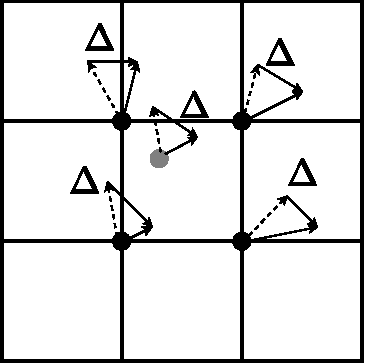
\includegraphics[width=0.4\textwidth]{Grid2Particle.pdf}
    \caption{Para atualizar a velocidade inicial da partícula (cinza), representada pela linha tracejada, usa-se a interpolação das diferenças das velocidades final e inicial, dada por $\Delta$, nos pontos da grade (pretos).}
    \label{fig:transfercellparticle}
\end{figure}

% [TODO] Apresentação do PIC, passos, explicar transferências grade-partícula, e então o uso de diferenças finitas para calcular os operadores diferenciais na grade.
%Avaliação qualitativa!

\section{Aspectos de Implementação}
\label{sec:implementation}
Para o desenvolvimento do solucionador FLIP, usou-se a linguagem C++17. Como implementação base usou-se a biblioteca CG, desenvolvida para a disciplina de Computação Gráfica. Para controlar o programa via interface gráfica a biblioteca ImGui \cite{ImGui} foi adotada e, por fim, como solucionador de sistemas lineares em matrizes esparsas utilizou-se o módulo \textit{Sparse} da biblioteca de álgebra linear Eigen \cite{eigenweb}.

A implementação conta com o uso de orientação a objetos para a composição das classes necessárias para o solucionador FLIP. Estas são apresentadas nas Figuras \ref{fig:solvershierarchy}, \ref{fig:gridfluidsolver} e \ref{fig:picsolver}, a \figref{fig:solvershierarchy} apresenta a hierarquia de classes que parte de \texttt{PhysicsAnimation} e com subsequentes especializações alcança \texttt{FlipSolver}. A classe base \texttt{PhysicsAnimation} provém aos seus objetos armazenar informações gerais de uma simulação baseada em física, como o tempo decorrido desde o início da simulação e também o número de quadros passados. Além disso fornece duas maneiras de subdividir o passo de tempo da simulação e então executar seu avanço, a primeira maneira sendo uma subdivisão fixa em $n$ passos menores e a outra uma divisão adaptativa onde toma-se o resultado de um método, substituível pelas classes derivadas, para subdividir o passo de tempo.

\begin{figure}[ht]
    \centering
    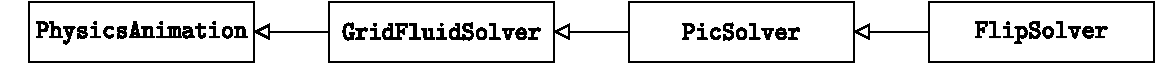
\includegraphics[width=\textwidth]{Solvers.pdf}
    \caption{Hierarquia de classes dos solucionadores.}
    \label{fig:solvershierarchy}
\end{figure}

Em seguida, a classe \texttt{GridFluidSolver} e as principais classes relacionadas a ela podem ser observadas na \figref{fig:gridfluidsolver}. Esta representa a implementação de um solucionador Euleriano e como tal, armazena o campo velocidade e computa os termos das equações de Navier-Stokes em uma grade. Para armazenar a velocidade, foi utilizada a classe \texttt{FaceCenteredGrid} que contém a implementação de uma grade regular centrada em face, ou seja, com pontos de controle nos centros das faces das células. Além desta, para determinar as propriedades dos fluidos temos três classes associadas a \texttt{GridFluidSolver}, são elas
\texttt{GridBackwardEulerDiffusionSolver}, classe que implementa o método de Euler implícito para determinar a força viscosa, \texttt{GridFractionalSinglePhasePressureSolver}, que realiza o cômputo da pressão do fluido, e por fim,  \texttt{GridFractionalBoundaryConditionSolver}, encarregada de computar as condições de contorno como interações com outros corpos e com os limites do espaço de simulação. É importante ressaltar que para o funcionamento correto de um solucionador Euleriano como o descrito acima, se faz necessário solucionar o passo de advecção, ou transferência de matéria, na grade. Como o propósito de \texttt{GridFluidSolver} é servir de base comportamental para as subsequentes classes derivadas e também os solucionadores PIC e FLIP solucionam advecção com uso de partículas, o passo de advecção na grade não foi implementado e portanto, não será abordado nessa seção.

\begin{figure}[ht]
    \centering
    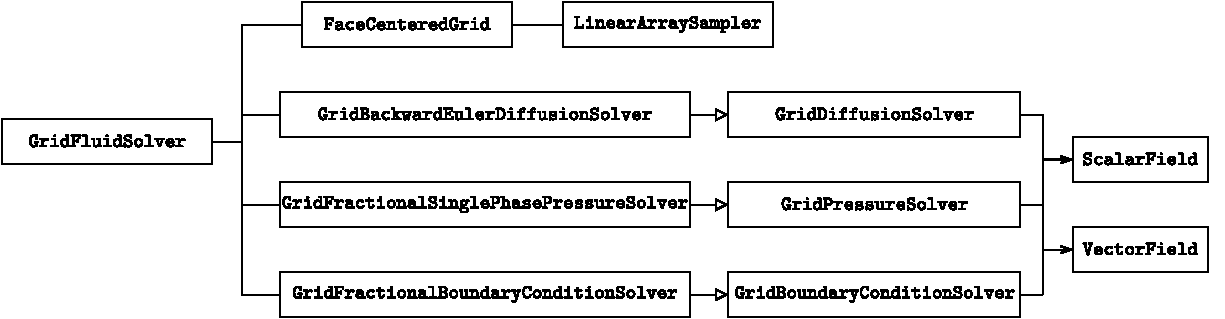
\includegraphics[width=\textwidth]{GridFluidSolverDiagram.pdf}
    \caption{Classe \texttt{GridFluidSolver} e principais classes relacionadas.}
    \label{fig:gridfluidsolver}
\end{figure}

A \figref{fig:facecenteredgrid} ilustra o caso bidimensional de uma grade centrada em face de ordem três, tal como implementada em \texttt{FaceCenteredGrid}. Nota-se que a velocidade tem suas componentes $x$ e $y$ armazenadas nos eixos horizontal e vertical respectivamente, além disso, para cada componente a grade armazena mais células na direção positiva da componente, com isso, elas podem ser vistas como grades 4x3 para a componente $x$ e 3x4 para $y$. A motivação por trás do uso da grade centrada em face é que esta não origina o problema chamado \textit{odd-even decoupling}, causando a introdução de valores não físicos para as propriedades do fluido, em especial a pressão, mais detalhes sobre o problema e sua solução podem ser encontrados em \cite{RAUWOENS200779}. Com a grade centrada em face é possível determinar, com uso de interpolação, as velocidades tanto no centro das células quanto nos seus cantos, bastando tomar os pontos corretamente para seu cômputo. Para tanto, diversos tipos de interpolação podem ser adotadas, por sua simplicidade de implementação e também por apresentar resultados aceitáveis adotou-se a interpolação linear, posteriormente implementada por \texttt{LinearArraySampler}, sua associação com \texttt{FaceCenteredGrid} permite aos seus objetos interpolarem a velocidade em qualquer ponto da grade. As classes responsáveis por calcular as propriedades dos fluidos dependem de \texttt{ScalarField} e \texttt{VectorField}, estas são classes abstratas que modelam os comportamentos essenciais de campos escalares e vetoriais, como avaliar o campo para um dado ponto no espaço ou obter o divergente para este ponto, respectivamente.

\begin{figure}[ht]
    \centering
    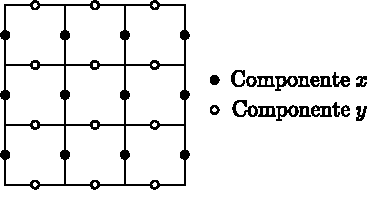
\includegraphics[width=0.5\textwidth]{FaceCenteredGrid.pdf}
    \caption{Exemplo de uma grade regular centrada em face, as componentes da velocidade são armazenadas separadamente.}
    \label{fig:facecenteredgrid}
\end{figure}

A classe \texttt{GridBackwardEulerDiffusionSolver}, derivada de \texttt{GridDiffusion-\linebreak Solver}, implementa o método de Euler implícito para solucionar o termo $c$ da \eqnref{eq:momentum2}, a viscosidade do fluido. Com o método de Euler adotado, a novo velocidade é calculada por sistemas lineares da forma $A \cdot x = b$ para cada componente da velocidade, para solucionar esse sistema utiliza-se a implementação do Gradiente Conjugado \cite{Hestenes&Stiefel:1952} em \texttt{Eigen::ConjugateGradient}. A matriz $A$ de cada sistema é uma matriz simétrica montada da seguinte forma: mapeia-se cada ponto na grade para uma linha da matriz, caso este ponto contenha fluido, sua linha correspondente conterá $-c$ nas colunas representando células vizinhas e $kc + 1$ para a diagonal, onde $k$ é o número de células vizinhas que não estão fora dos limites e $c = \frac{\Delta t \mu }{\Delta h^2}$, em que $h$ é o tamanho da célula na referente componente. Para que o método de Euler suporte o uso das condições de contorno de Newmann e de Dirichlet, estas são incluídas na matriz do sistema linear implicitamente.

% Falar da classe base abstrata, a classe derivada implementa as condições de borda, abordar as condições de borda.

A classe \texttt{GridFractionalBoundaryConditionSolver}, derivada da classe abstrata \texttt{GridBoundaryConditionSolver}, é encarregada de restringir o campo velocidade do fluido com as condições de contorno \textit{no-flux}, e \textit{free/no-slip} conforme Equações \eqref{eq:noflux} e \eqref{eq:slipcond}. O termo \texttt{Fractional} presente no nome da classe indica que para determinar a fronteira de um colisor esta calcula para cada célula da grade, a fração de sua área (ou volume no caso tridimensional) tomada pelo colisor, desta maneira, se um sólido ocupa metade de uma célula, a fração desta célula será $0.5$. Um exemplo deste método proposto por Batty et al \cite{BattyFastVariational} encontra-se na \figref{fig:fractionalBoundary}, nela é possível ver que para determinar a fração da célula tomada pelo colisor, avaliam-se os pontos vizinhos a uma distância de meia célula. Essa abordagem se opõe a simplesmente marcar a célula de forma binária, ou contendo fluido ou tomada pelo colisor.

\begin{figure}
    \centering
    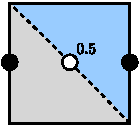
\includegraphics[width=0.3\textwidth]{FractionalGrid.pdf}
    \caption{Método fracionário para determinar interface fluido-sólido. O ponto central indica a fração da célula tomada por sólido (cinza) avaliando os pontos vizinhos, em sólido ou fluido (azul). Adaptado de \cite{BattyFastVariational}.}
    \label{fig:fractionalBoundary}
\end{figure}


A classe responsável por computar a pressão é \texttt{GridFractionalSinglePhase-\linebreak PressureSolver}. Da mesma maneira que \texttt{GridFractionalBoundaryConditionSol-\linebreak ver}, esta utiliza frações para determinar porções de fluido em uma célula. Em adição, considera-se um fluido monofásico e portanto, células que não contenham fluido são tratadas como atmosféricas, preenchidas por ar, desta maneira a pressão fora do fluido será constante e o campo velocidade não será alterado nessas regiões. Para determinar a força proveniente da pressão, a classe computa o gradiente da pressão, conforme termo $b$ da \eqnref{eq:momentum2} e, assim como o solucionador de viscosidade, usa o método de Euler implícito para calcular essa pressão. Com o método de Euler implícito agrega-se a \eqnref{eq:pressure} ao gradiente da pressão para obter um sistema linear chamado Equação de Pressão de Poisson (EPP) cuja solução fornece a pressão que mantém o campo velocidade com divergente nulo ($\nabla \cdot \Vec{u} = 0$), novamente a implementação do Gradiente Conjugado em \texttt{Eigen::ConjugateGradient} é utilizada para solucionar esse sistema linear. Para determinar a matriz de coeficientes $A$ e vetor $b$ adotou-se a implementação em \cite{fluidcoupling07}. Por fim, após obter-se a solução do sistema, calcula-se o gradiente da pressão e este é transferido para a grade.

Por fim, outro aspecto importante introduzido em \texttt{GridFluidSolver} é o número de Courant–Friedrichs–Lewy (CFL) \cite{cflnumber}, em termos gerais, este parâmetro é utilizado para subdividir o espaço de tempo e então garantir que uma partícula nunca ira atravessar mais que uma célula da grade em uma iteração. Em uma grade $\mathbf{F}$ esse valor é dado por
\begin{equation}
    C = \frac{v \cdot \Delta t}{\min \{ \Delta x, \Delta y \}},   
\end{equation}
no caso bidimensional onde, $v$ é a maior componente de
\begin{equation}
    \max_{\forall (i, j) \in \mathbf{F}} \{\Vec{u}_{i, j} = \Vec{u}^c_{i, j} + \Delta t \cdot \Vec{g}\},
\end{equation}
sendo $\Vec{u}^c_{i, j}$ o valor da velocidade no centro da célula $(i, j)$, $\Vec{g}$ a gravidade e $\Delta t$ o passo de tempo que se deseja subdividir.

Tendo em vista o enunciado, é possível observar que \texttt{PicSolver} deriva de \texttt{Grid-\linebreak FluidSolver} para aproveitar o cômputo das propriedades do fluido na grade. Porém, algumas adaptações, abordadas posteriormente, devem ser feitas para  lidar com as interfaces grade-partícula, observando a \figref{fig:picsolver} vemos as relações de \texttt{PicSolver}, as primeiras são com \texttt{ParticleSystem}, classe que representa um sistema de partículas que armazena para cada partícula, posição e velocidade, e \texttt{ParticleEmitter}, a classe responsável pela emissão de partículas na simulação.

\begin{figure}[ht]
    \centering
    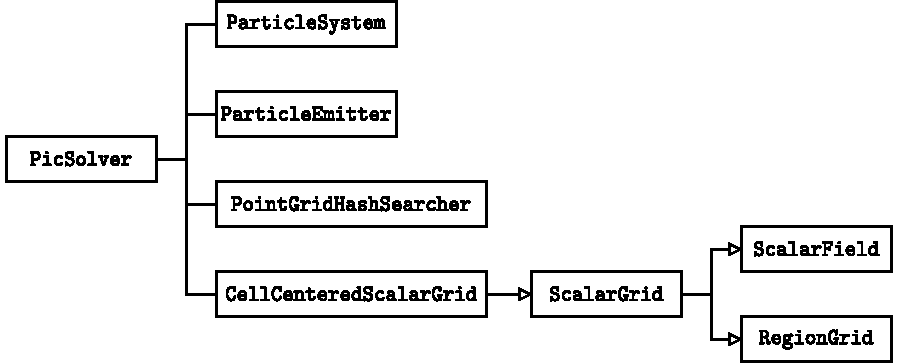
\includegraphics[width=\textwidth]{PicSolver.pdf}
    \caption{Classe \texttt{PicSolver} e suas relações.}
    \label{fig:picsolver}
\end{figure}

Uma das operações mais importantes em simulações que usam partículas é a busca de partículas próximas a um ponto no espaço. Pela própria natureza dos fluidos, é impossível estabelecer qualquer conectividade duradoura entre as partículas, por conta disso, esta é atualizada continuamente ao longo do tempo. Por esses motivos, é desejável que o processo de busca tome a menor quantidade de tempo possível, a proposta para tal é o uso de uma estrutura de aceleração com \textit{hashing} para encontrar as partículas vizinhas. A implementação desta estrutura encontra-se em \texttt{PointGridHashSearcher}, esta toma para sua criação um tamanho de célula, que deve ser maior ou igual a duas vezes o maior raio de busca. Possui também uma grade de lista de pontos, onde uma consulta dado um ponto no espaço fornece, com o uso de uma função espacial de \textit{hashing}, a lista de pontos próximos e, com esta lista em mãos, pode-se então realizar verificações de distância para restringir a partículas em um determinado raio de busca. A \figref{fig:gridhashsearcher} apresenta visualmente a busca de partículas vizinhas a um ponto marcado com \textbf{x} em um dado raio de busca.

\begin{figure}[ht]
    \centering
    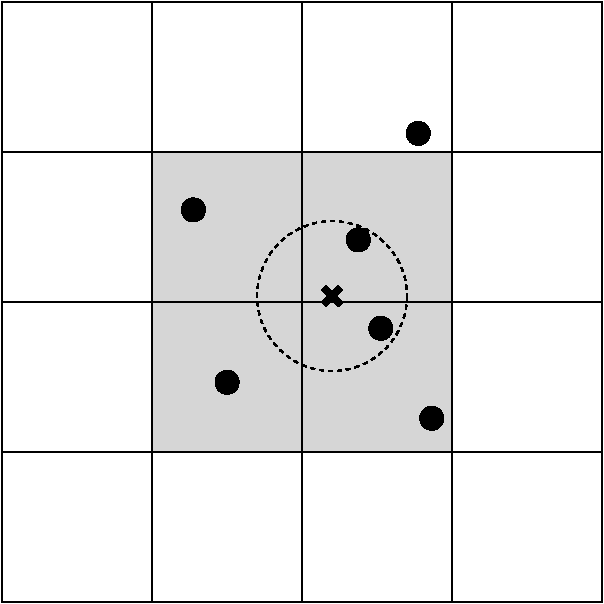
\includegraphics[width=0.4\textwidth]{PointGridHashSearcher.pdf}
    \caption{Busca de partículas vizinhas ao ponto marcado com \textbf{x} em um dado raio representado pela linhas tracejada, apenas as células em cinza são avaliadas. Posteriormente, distancia das partículas em cada célula cinza para o ponto determinam se elas estão ou não no raio de busca. Adaptado de \cite{kim_2017}.}
    \label{fig:gridhashsearcher}
\end{figure}

Os solucionadores de pressão, viscosidade e de condições de contorno usam campos escalares chamados \textit{signed distance field} (SDF) para determinar regiões ocupadas por fluido ou por sólidos, esses campos em geral avaliam valores negativos para pontos interiores a superfície e positivos para pontos exteriores. Pela dificuldade de determinar um SDF do fluido via função contínua, adota-se uma discretização deste campo escalar armazenado com uso de uma grade regular centrada em célula, implementada em \texttt{CellCenteredScalarGrid}. O campo escalar é calculado conforme implementação em \cite{kim_2017}, considerando $h$ a maior dimensão de uma célula da grade, para cada célula, o valor do campo no seu centro é $d - r$, onde $d$ é a distância do centro da célula até a partícula mais próxima (determinada com uso de \texttt{PointGridHashSearcher}) e $r = 1.2h/\sqrt{2}$ metade do raio de busca.

Além do abordado acima para \texttt{PicSolver}, este também realiza, antes e depois dos procedimentos de \texttt{GridFluidSolver}, as transferências de partícula para grade e de grade para partícula, respectivamente, exatamente como enunciado na \ssecref{ssec:hibridmethods}. Os passos de transferência adotam sempre uma influência local das grandezas, ou seja, as partículas, no passo de transferência de partícula para grade, levam suas velocidades para os pontos de controle nas células em que estão espacialmente contidas e, as células da grade, transferem a velocidade de volta para as partículas que nela estão.

Por último, a classe \texttt{FlipSolver} deriva de \texttt{PicSolver} e modifica os passos de transferência da seguinte maneira: ao fim da transferência de partículas para grade, armazena-se uma cópia desta grade com suas respectivas velocidades e então, no passo de transferência de grade para partículas, uma partícula tem sua velocidade incrementada com a diferença entre a velocidade atual na grade e a velocidade armazenada anteriormente.

% Para esta seção: essa aplicação usa C++17, usando Eigen e ImGui (ref). Usa como base a biblioteca de CG. Descrever componentes (diagrama de classes). Visão geral dos componentes em vista da funcionalidade. 2/3 diagramas de classe. Mencionar o CFL


\section{Resultados}
\label{sec:results}

Esta seção destina-se à apresentação dos resultados obtidos com a implementação do solucionador FLIP. Estes resultados são \textit{frames} de quatro simulações, na qual cada uma apresenta a evolução do fluido, cada simulação conta com: um posicionamento inicial do fluido, ao qual chama-se cena, viscosidade e pressão do fluido. As cenas escolhidas foram: \textit{Dam Breaking}, \textit{Double Dam Breaking} e \textit{Water Drop}. A primeira cena, \textit{Dam Breaking} (DB) consiste numa coluna de fluido que, sob ação da gravidade, cai sobre o chão. Como o próprio nome enuncia, esta cena pode representar o rompimento de uma barragem, liberando o escoamento do fluido. Em sequência, \textit{Double Dam Breaking} (DDB) é uma cena similar a \textit{Dam Breaking}, contando agora com duas colunas de fluido, uma em cada extremo do espaço de simulação, que sob ação da gravidade escoam em direções opostas até se chocar. Por fim, a cena \textit{Water Drop} (WD) ilustra uma circunferência de fluido acima de uma camada de fluido em repouso, sob ação da gravidade esta circunferência cai sobre o fluido interrompendo seu repouso e causando o efeito de uma gota caindo em um pequeno nível de líquido. Os experimentos foram realizados em um computador com processador AMD Ryzen-7 e 8 GB de memória RAM, o processo de visualização das simulações foi feita por um programa OpenGL simples que desenha esferas para representar as partículas, já que o objetivo é reservado a evidenciar o comportamento do fluido e não renderizá-lo.

A parametrização e as informações referentes a cada simulação encontram-se na \tabref{tab:simparams}. Nesta tabela tem-se $n$ como o número de partículas, $n_c$ o número de células da grade regular, $t$ o tempo de simulação em segundos e $F$ o número de \textit{frames} obtidos. Além dos dados sobre a simulação, tem-se também os referentes as propriedades do fluido como coeficiente de viscosidade, representado por $\mu$ e densidade, dada por $\rho$. Enfim, para todas as simulações usou-se um espaço de simulação definido por um quadrado de lado dois metros, uma grade regular de 200 por 200 e um esquema adaptativo de subdivisão do passo de tempo conforme enunciado na \secref{sec:implementation}. Uma grade 200 por 200 em um espaço de $4m^2$ gera células quadradas de lado $0.01$, as justificativas para o uso de uma grade de granularidade fina como esta são ligadas a qualidade da avaliação das derivadas parciais, como evidenciado na \ssecref{ssec:fundamentals} e no fato de que, com mais pontos de controle registrando a velocidade do fluido, diminui-se a introdução de viscosidade artificial, tornando a simulação mais estável para maiores tempos de simulação.

\begin{table}[ht]
\centering
\begin{tabular}{|l|c|c|c|c|c|}
\hline
Cena & \textit{n} & \textit{t} & \textit{F} & $\mu$ & $\rho$ \\ \hline
DB   & 10500      & 78         & 480        & 0     & 1      \\ \hline
DB   & 10500      & 91         & 480        & 0.05  & 1      \\ \hline
DDB  & 22051      & 99         & 480        & 0     & 1      \\ \hline
WD   & 25073      & 126        & 480        & 0     & 1      \\ \hline
\end{tabular}
\caption{Números e parâmetros das simulações.}
\label{tab:simparams}
\end{table}

As Figuras \ref{fig:dambreaking} e \ref{fig:viscdambreaking} apresentam, cada uma, \textit{frames} provenientes da simulação da cena \textit{Dam Breaking}, com uso de 10500 partículas de um fluido. A diferença entre as duas simulações é a viscosidade utilizada, para a da \figref{fig:dambreaking} o fluido é invíscido, isto é, tem viscosidade nula, por conta disso o fluido desta simulação se espalha facilmente em pequenos fragmentos ao colidir com as laterais direita e superior. Já para a \figref{fig:viscdambreaking}, o fluido possuí viscosidade de $0.05$, o que causa aparente diferença em seu comportamento, impedindo, por exemplo, a divisão em fragmentos que acontece na simulação anterior. Na \figref{fig:doubledb} tem-se a simulação de 22051 partículas na cena \textit{Double Dam Breaking}, as altas colunas de fluido invíscido colidem no centro e se espalham para o topo a medida que escorrem para baixo. Por fim, a \figref{fig:waterdrop} apresenta a cena \textit{Water Drop} com 25073 partículas, onde uma circunferência de fluido interrompe o repouso do líquido na base produzindo ondas.


\clearpage

\begin{figure}[!ht] \centering
	\begin{subfigure}[!h]{0.3\textwidth} \centering
		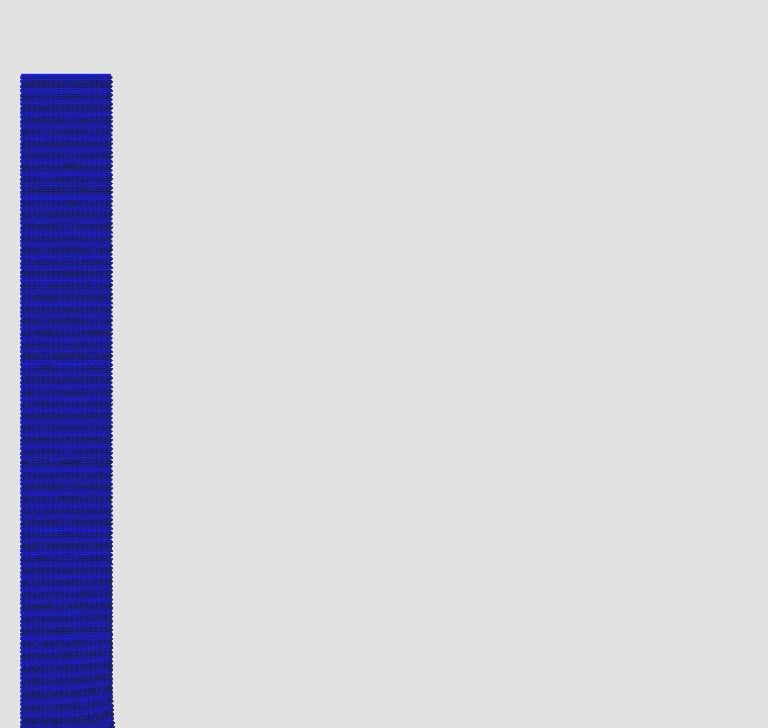
\includegraphics[width=\textwidth]{DB/DB-000.jpg}
	\end{subfigure}
    \begin{subfigure}[!h]{0.3\textwidth} \centering
		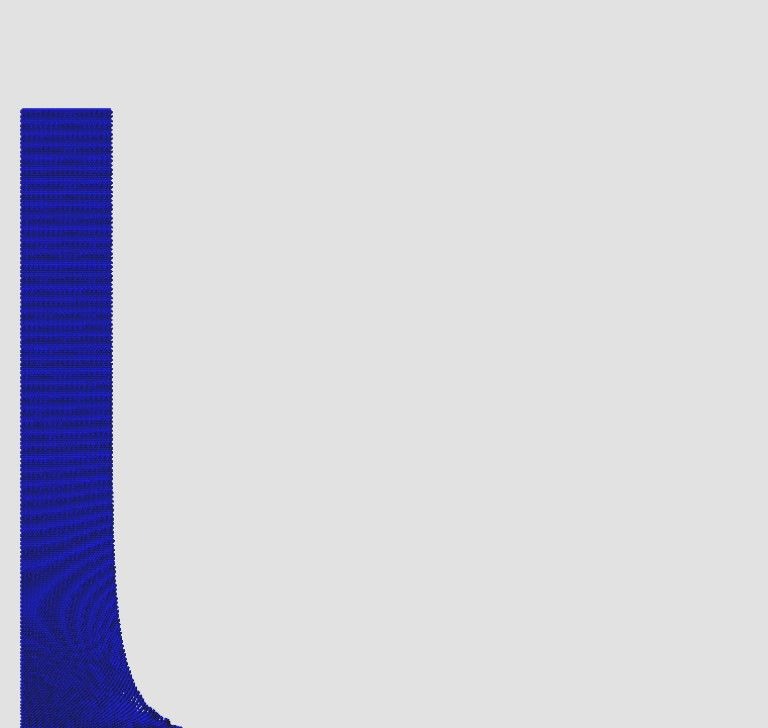
\includegraphics[width=\textwidth]{DB/DB-001.jpg}
	\end{subfigure}
	\begin{subfigure}[!h]{0.3\textwidth} \centering
		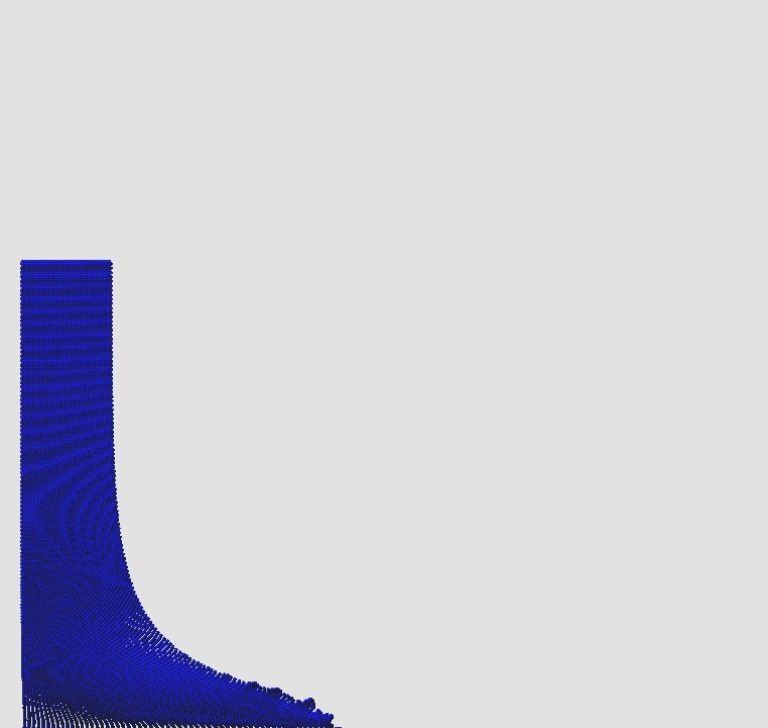
\includegraphics[width=\textwidth]{DB/DB-002.jpg}
	\end{subfigure}
	\begin{subfigure}[!h]{0.3\textwidth} \centering
		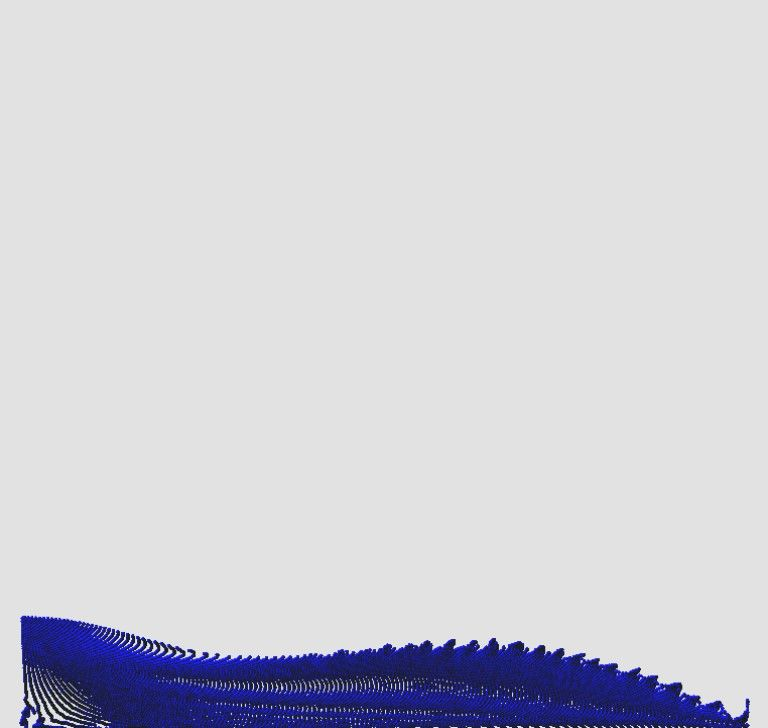
\includegraphics[width=\textwidth]{DB/DB-003.jpg}
	\end{subfigure}
	\begin{subfigure}[!h]{0.3\textwidth} \centering
		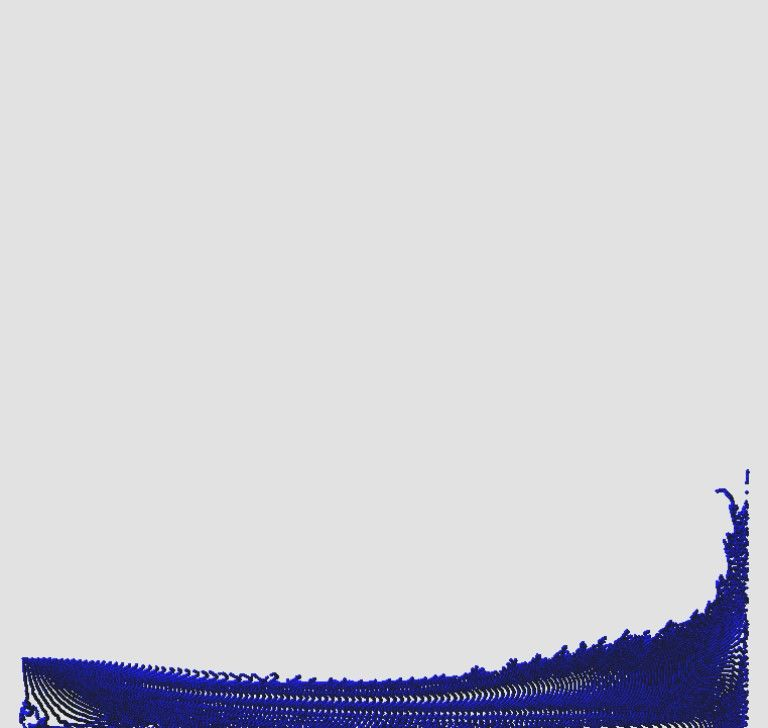
\includegraphics[width=\textwidth]{DB/DB-004.jpg}
	\end{subfigure}
	\begin{subfigure}[!h]{0.3\textwidth} \centering
		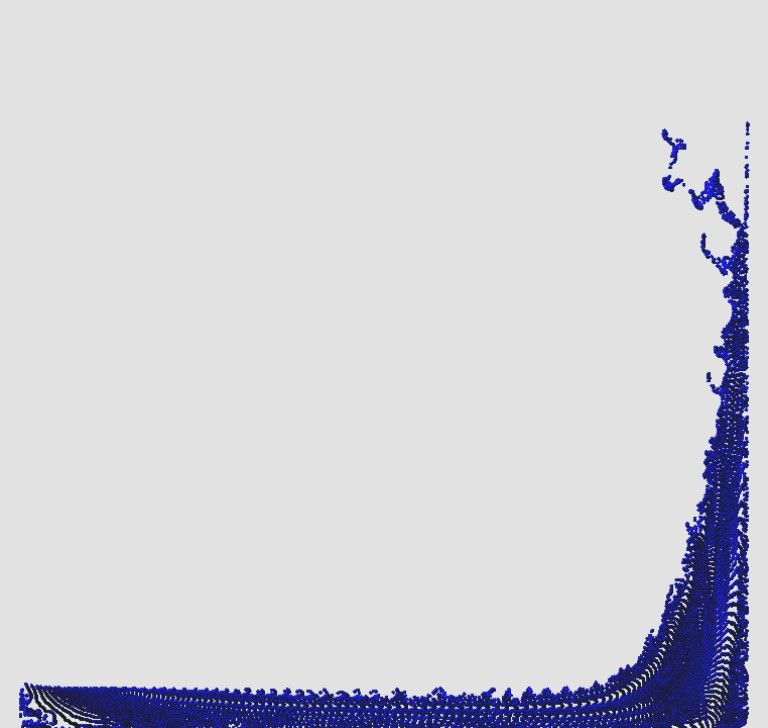
\includegraphics[width=\textwidth]{DB/DB-005.jpg}
	\end{subfigure}
	\begin{subfigure}[!h]{0.3\textwidth} \centering
		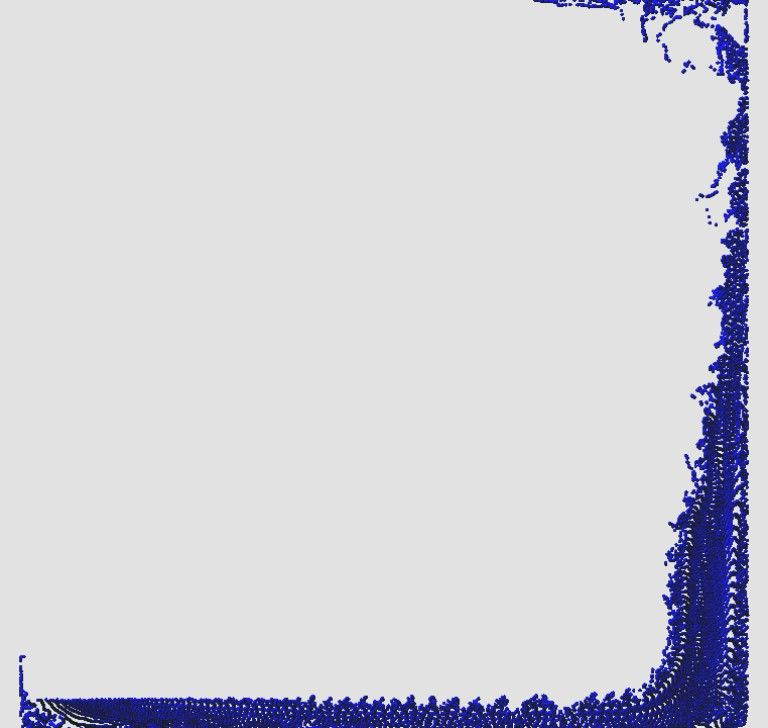
\includegraphics[width=\textwidth]{DB/DB-006.jpg}
	\end{subfigure}
	\begin{subfigure}[!h]{0.3\textwidth} \centering
		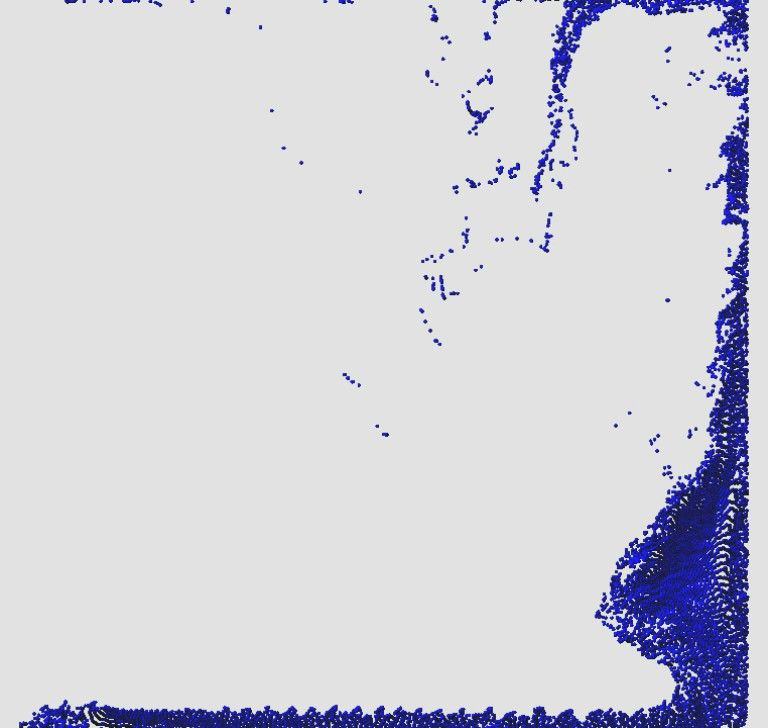
\includegraphics[width=\textwidth]{DB/DB-007.jpg}
	\end{subfigure}
	\begin{subfigure}[!h]{0.3\textwidth} \centering
		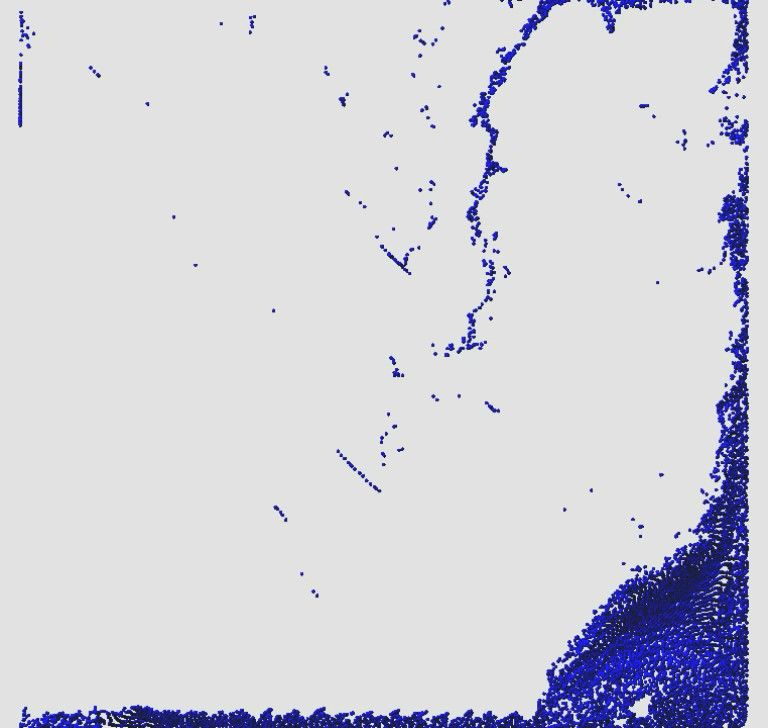
\includegraphics[width=\textwidth]{DB/DB-008.jpg}
	\end{subfigure}
	\begin{subfigure}[!h]{0.3\textwidth} \centering
		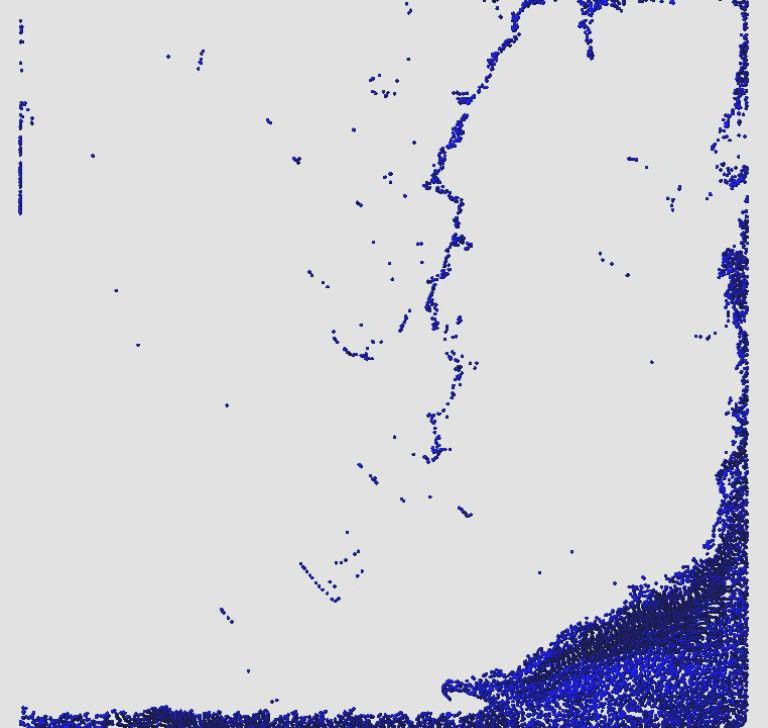
\includegraphics[width=\textwidth]{DB/DB-009.jpg}
	\end{subfigure}
	\begin{subfigure}[!h]{0.3\textwidth} \centering
		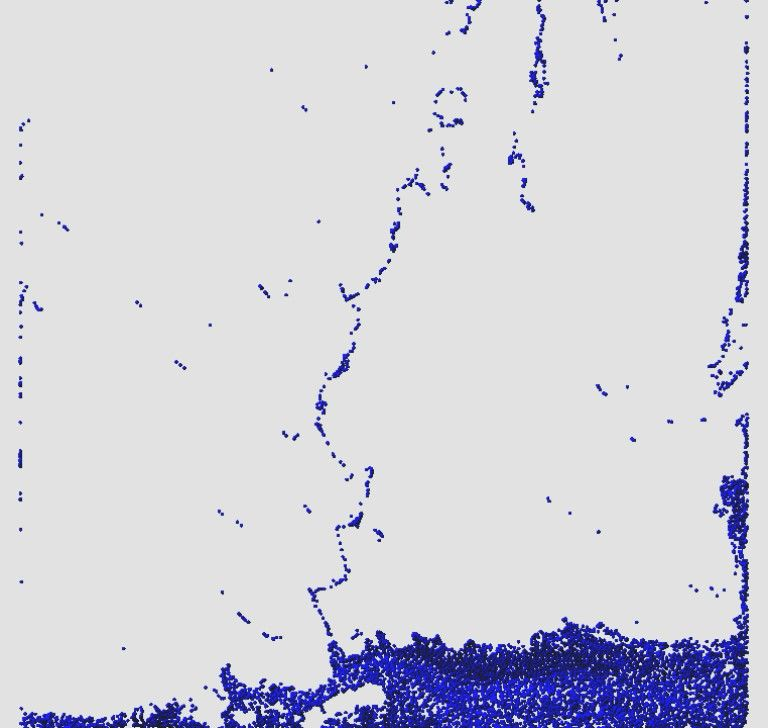
\includegraphics[width=\textwidth]{DB/DB-010.jpg}
	\end{subfigure}
	\begin{subfigure}[!h]{0.3\textwidth} \centering
		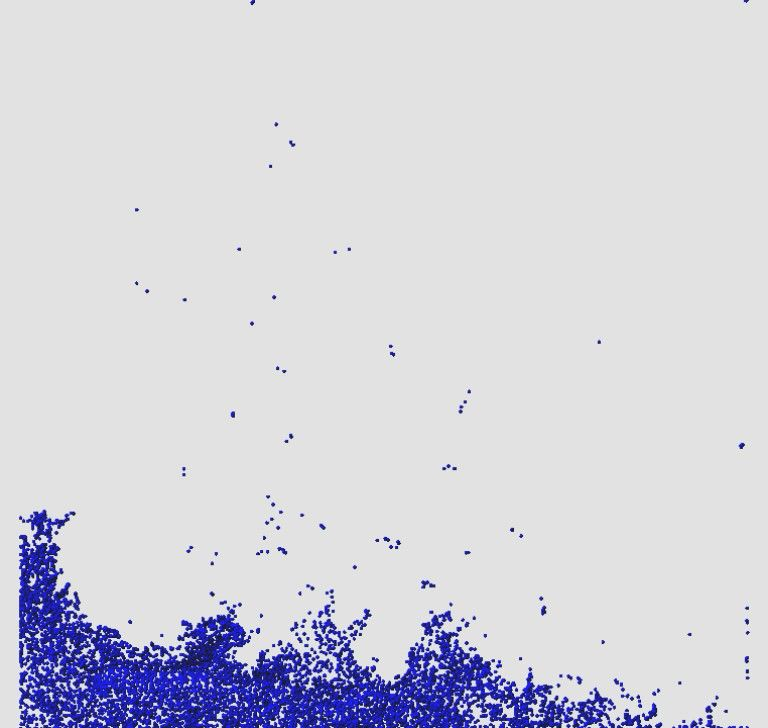
\includegraphics[width=\textwidth]{DB/DB-011.jpg}
	\end{subfigure}
    \caption{Simulação \textit{Dam Breaking} de um fluido invíscido.}
    \label{fig:dambreaking}
\end{figure}

\begin{figure}[!ht] \centering
	\begin{subfigure}[!h]{0.3\textwidth} \centering
		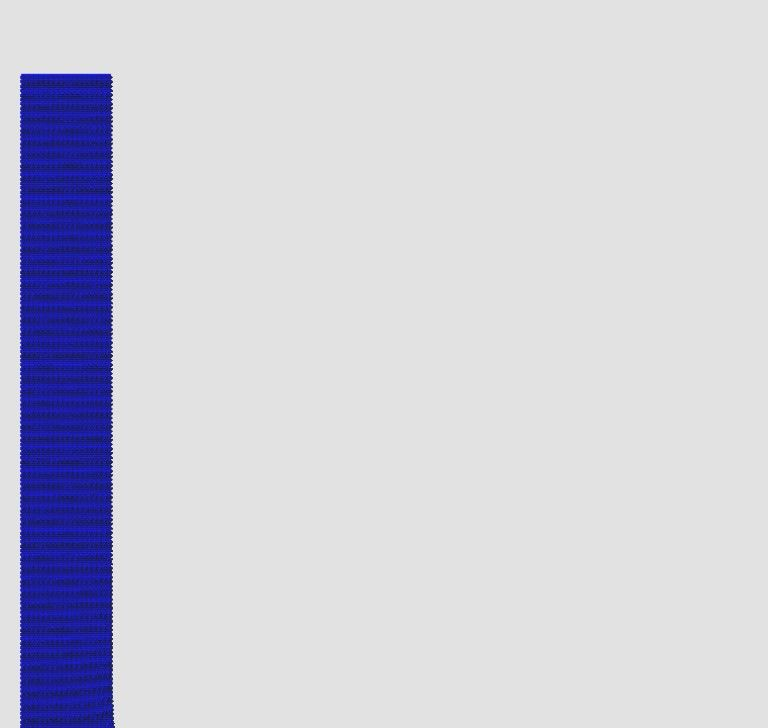
\includegraphics[width=\textwidth]{VDB/VDB-01.jpg}
	\end{subfigure}
    \begin{subfigure}[!h]{0.3\textwidth} \centering
		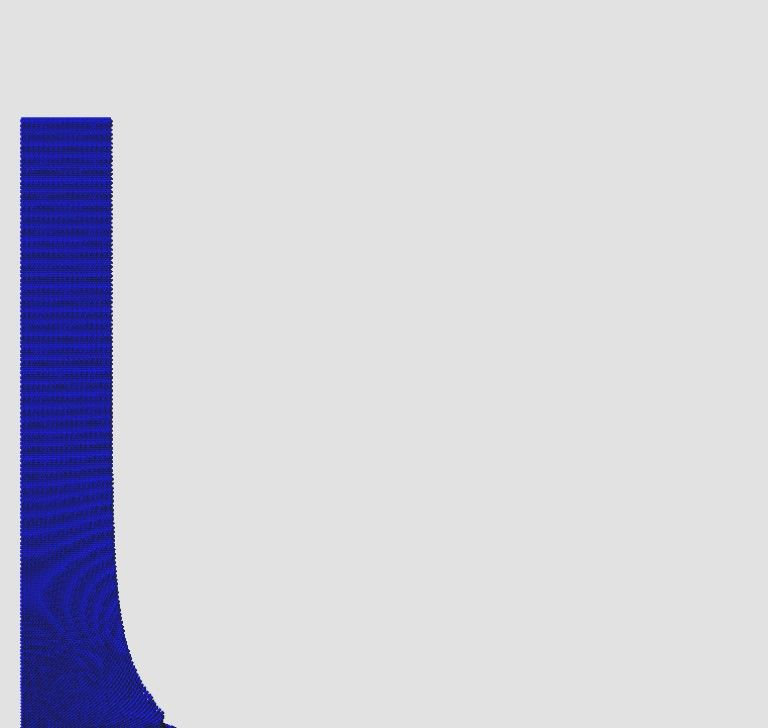
\includegraphics[width=\textwidth]{VDB/VDB-02.jpg}
	\end{subfigure}
	\begin{subfigure}[!h]{0.3\textwidth} \centering
		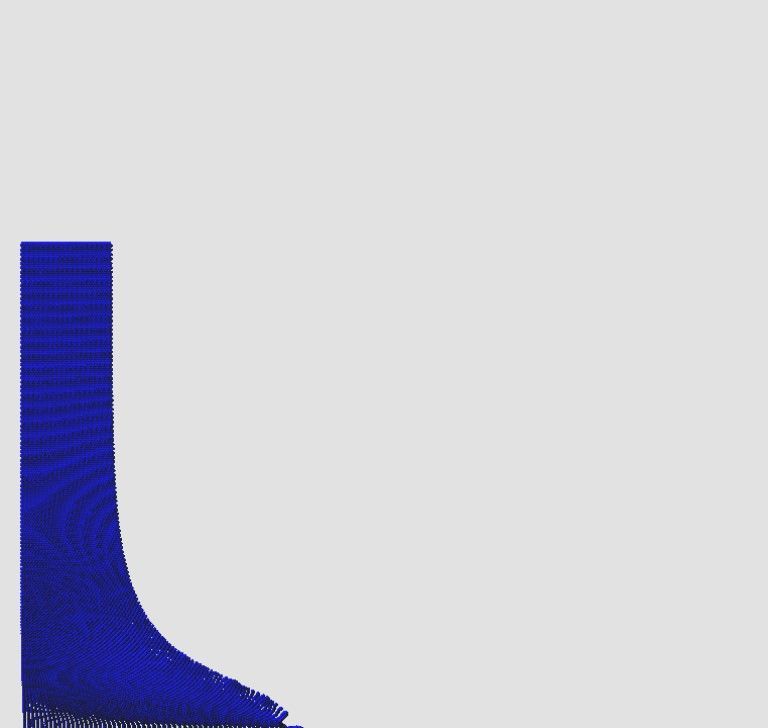
\includegraphics[width=\textwidth]{VDB/VDB-03.jpg}
	\end{subfigure}
	\begin{subfigure}[!h]{0.3\textwidth} \centering
		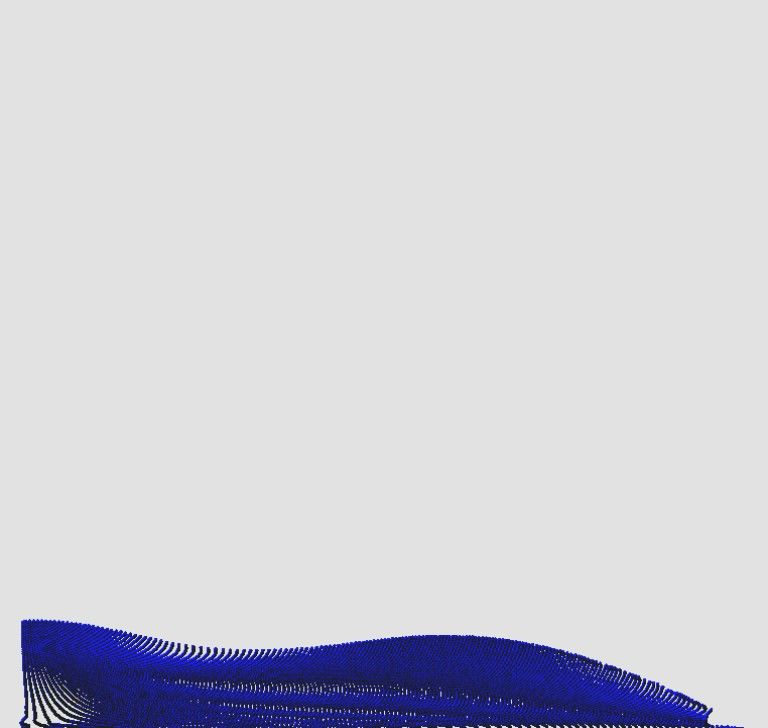
\includegraphics[width=\textwidth]{VDB/VDB-04.jpg}
	\end{subfigure}
	\begin{subfigure}[!h]{0.3\textwidth} \centering
		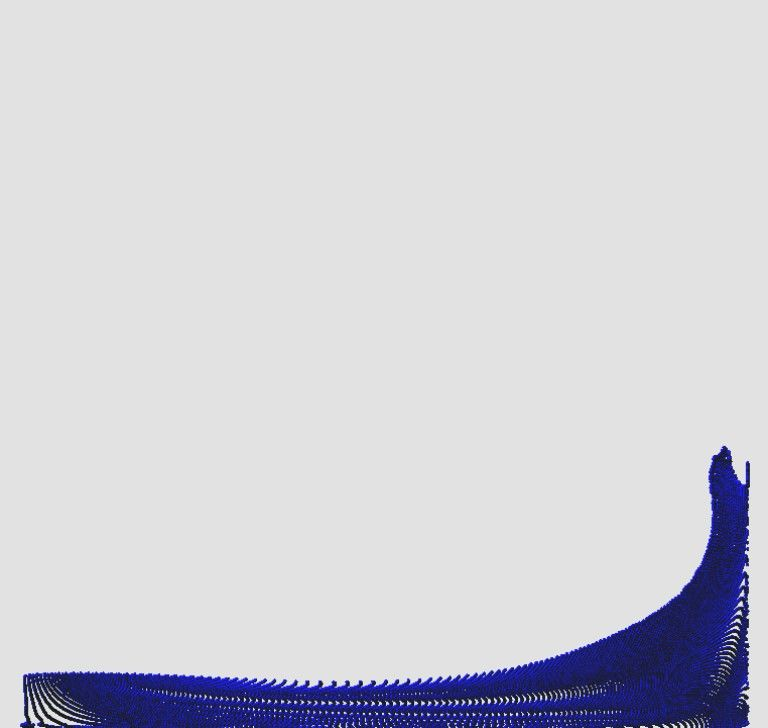
\includegraphics[width=\textwidth]{VDB/VDB-05.jpg}
	\end{subfigure}
	\begin{subfigure}[!h]{0.3\textwidth} \centering
		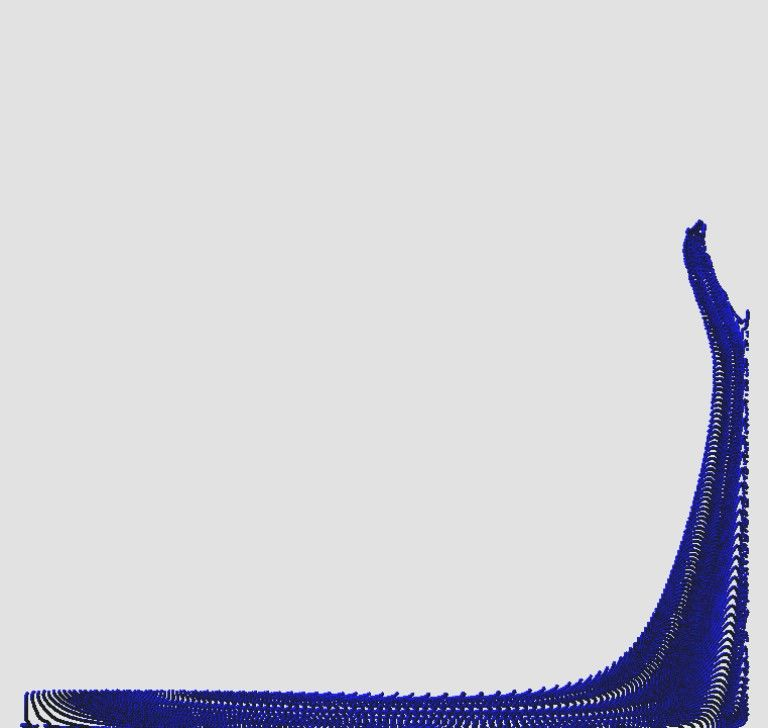
\includegraphics[width=\textwidth]{VDB/VDB-06.jpg}
	\end{subfigure}
	\begin{subfigure}[!h]{0.3\textwidth} \centering
		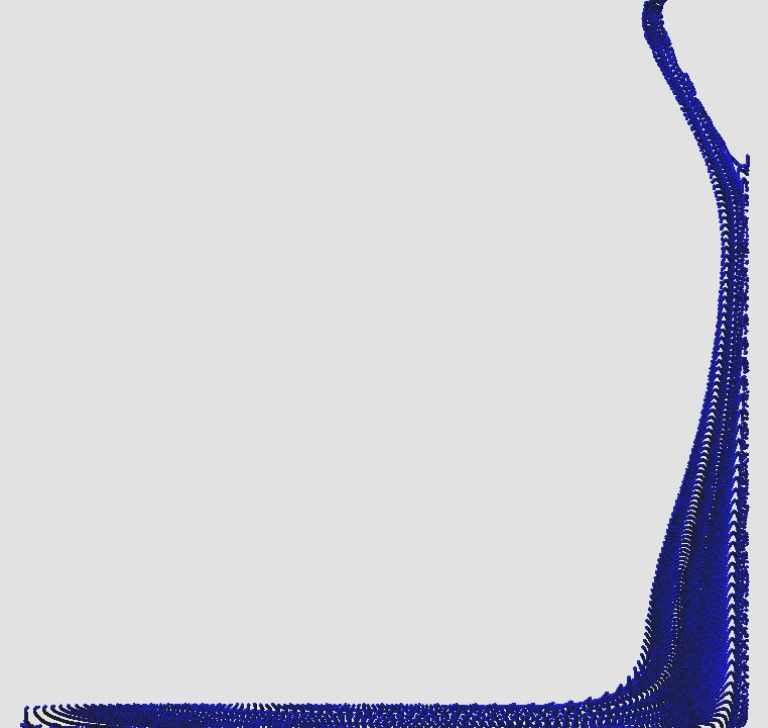
\includegraphics[width=\textwidth]{VDB/VDB-07.jpg}
	\end{subfigure}
	\begin{subfigure}[!h]{0.3\textwidth} \centering
		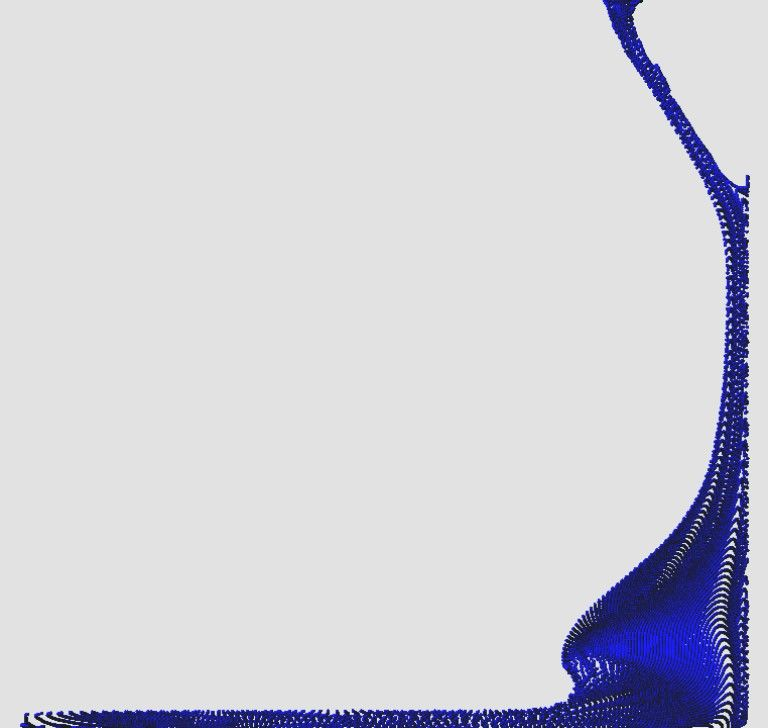
\includegraphics[width=\textwidth]{VDB/VDB-08.jpg}
	\end{subfigure}
	\begin{subfigure}[!h]{0.3\textwidth} \centering
		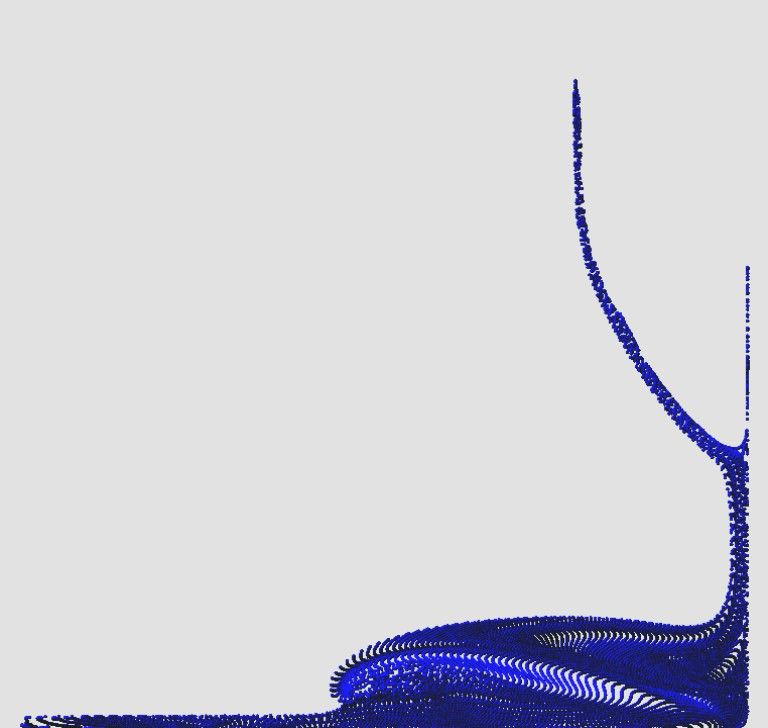
\includegraphics[width=\textwidth]{VDB/VDB-09.jpg}
	\end{subfigure}
	\begin{subfigure}[!h]{0.3\textwidth} \centering
		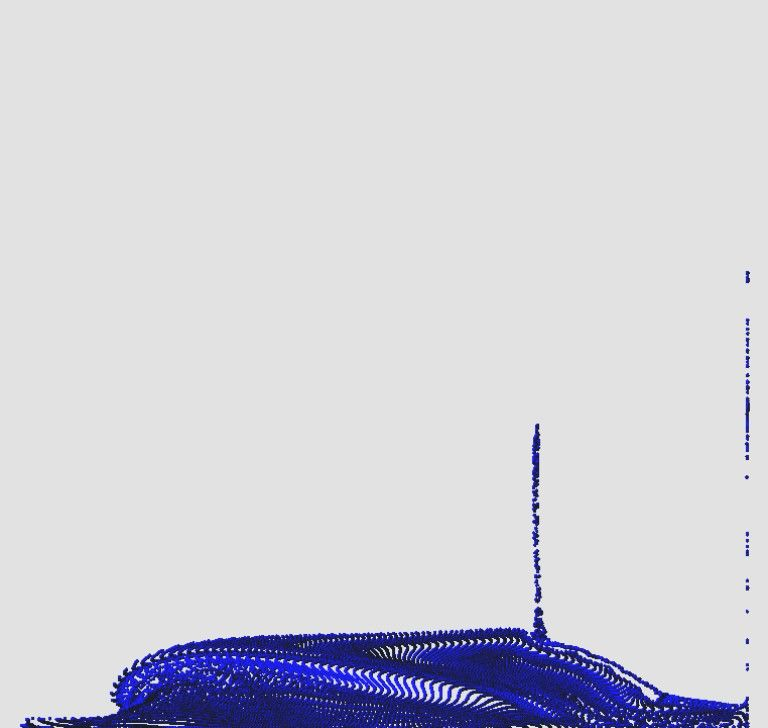
\includegraphics[width=\textwidth]{VDB/VDB-10.jpg}
	\end{subfigure}
	\begin{subfigure}[!h]{0.3\textwidth} \centering
		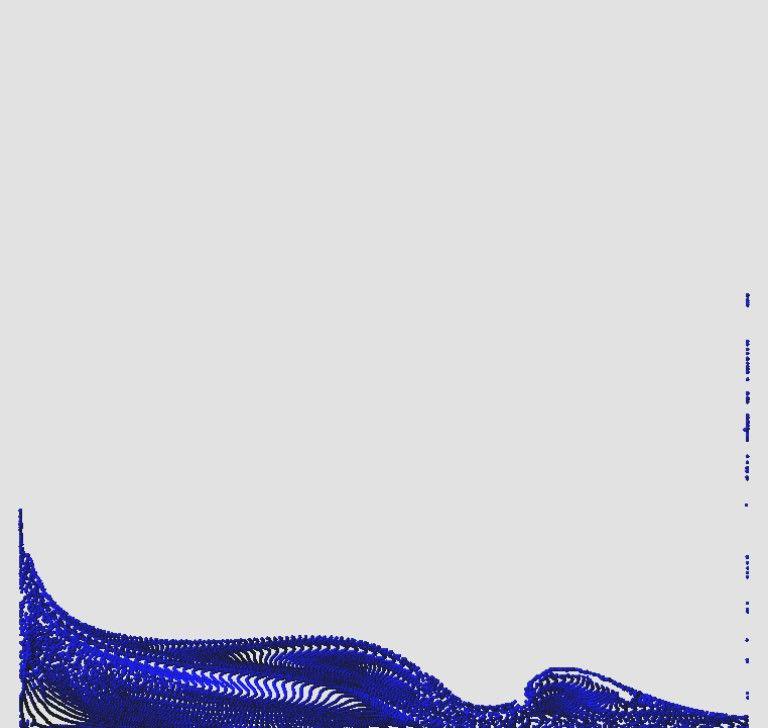
\includegraphics[width=\textwidth]{VDB/VDB-11.jpg}
	\end{subfigure}
	\begin{subfigure}[!h]{0.3\textwidth} \centering
		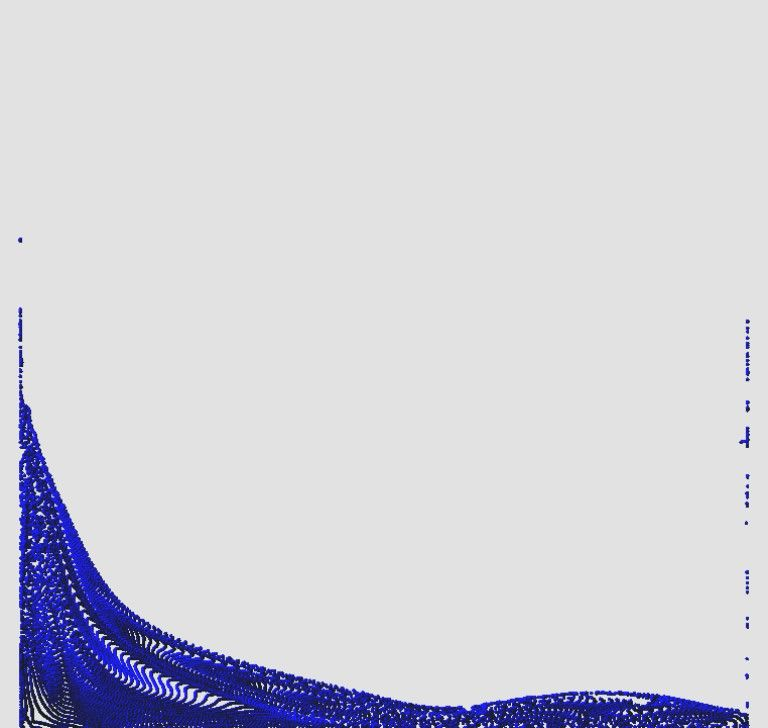
\includegraphics[width=\textwidth]{VDB/VDB-12.jpg}
	\end{subfigure}
    \caption{Simulação \textit{Dam Breaking} com viscosidade $0.05$.}
    \label{fig:viscdambreaking}
\end{figure}


\begin{figure}[!ht] \centering
	\begin{subfigure}[!h]{0.3\textwidth} \centering
		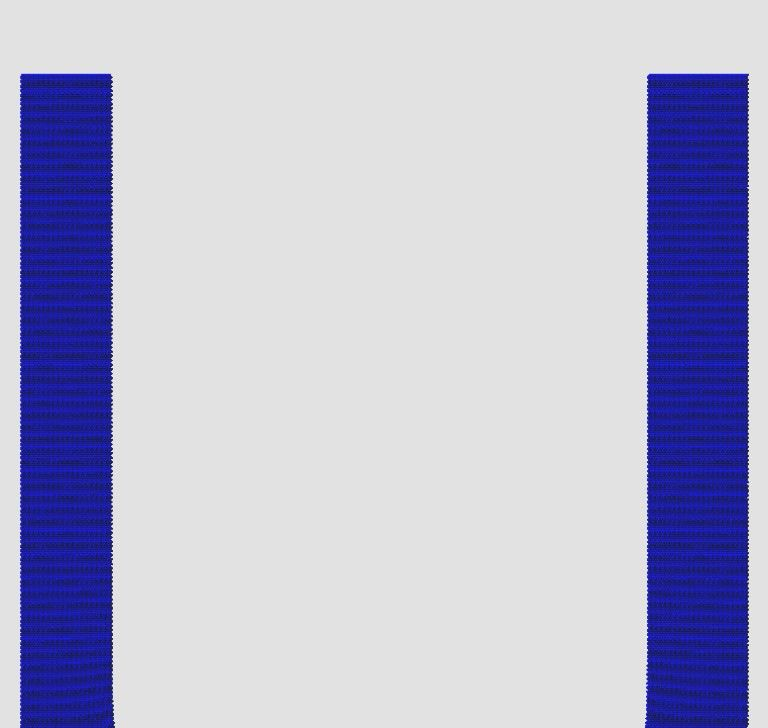
\includegraphics[width=\textwidth]{DDB/DDB-00.jpg}
	\end{subfigure}
    \begin{subfigure}[!h]{0.3\textwidth} \centering
		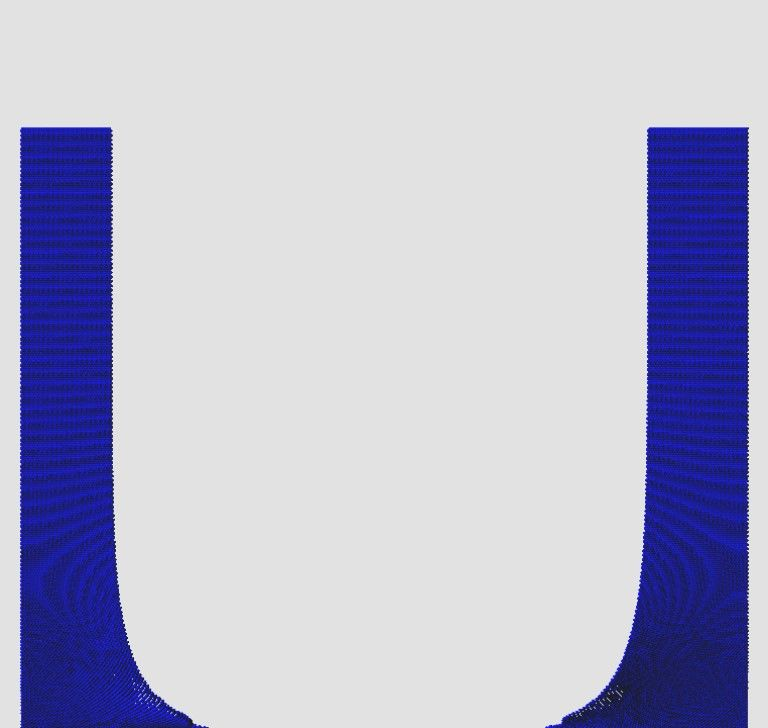
\includegraphics[width=\textwidth]{DDB/DDB-01.jpg}
	\end{subfigure}
	\begin{subfigure}[!h]{0.3\textwidth} \centering
		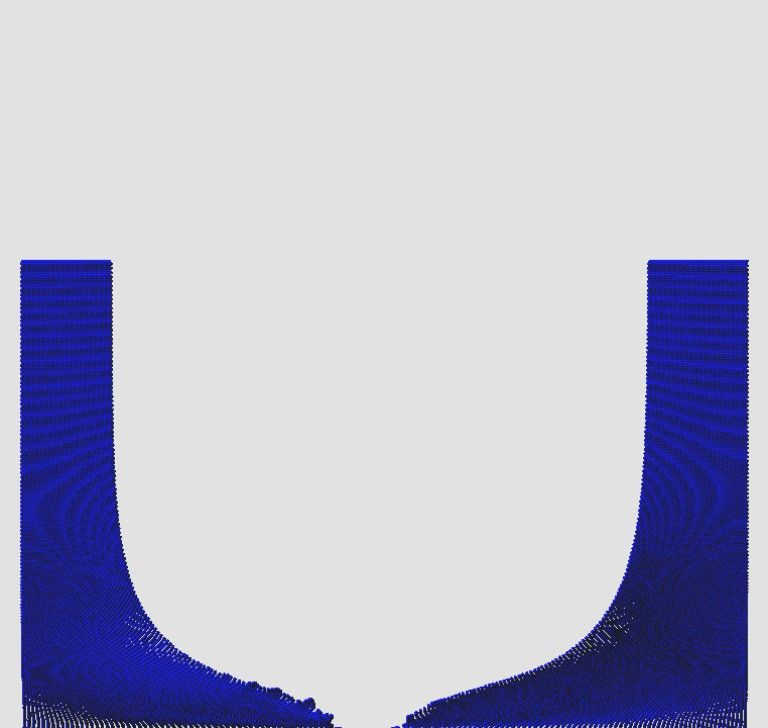
\includegraphics[width=\textwidth]{DDB/DDB-02.jpg}
	\end{subfigure}
	\begin{subfigure}[!h]{0.3\textwidth} \centering
		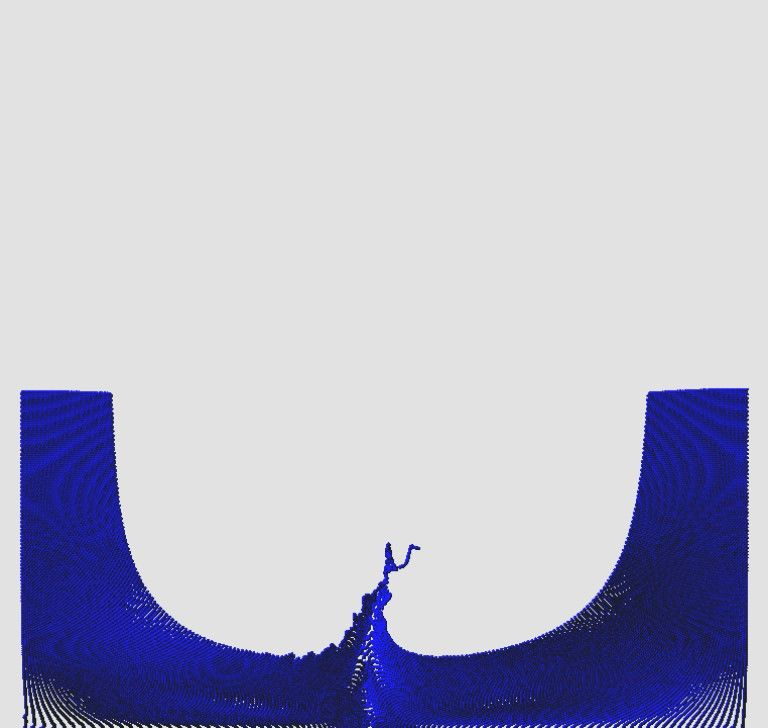
\includegraphics[width=\textwidth]{DDB/DDB-03.jpg}
	\end{subfigure}
	\begin{subfigure}[!h]{0.3\textwidth} \centering
		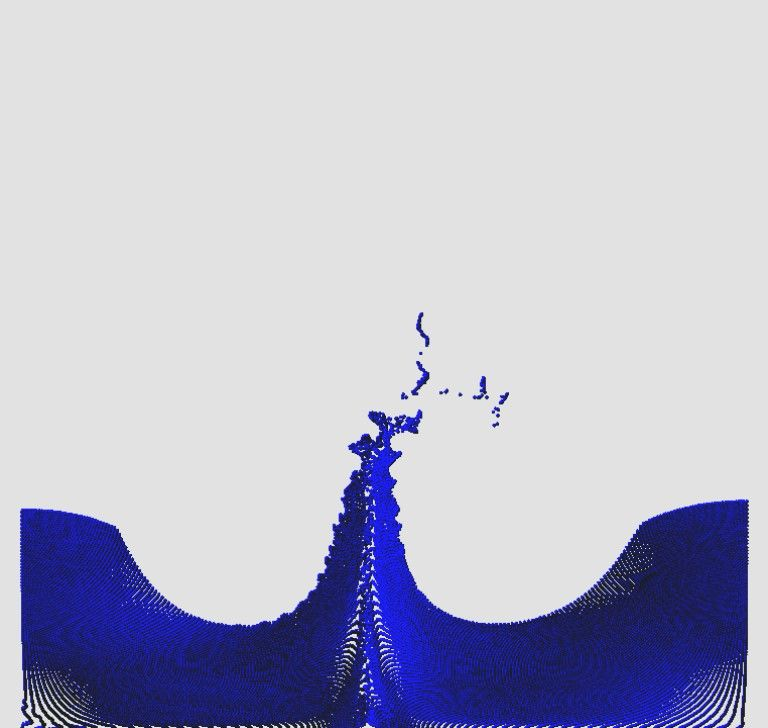
\includegraphics[width=\textwidth]{DDB/DDB-04.jpg}
	\end{subfigure}
	\begin{subfigure}[!h]{0.3\textwidth} \centering
		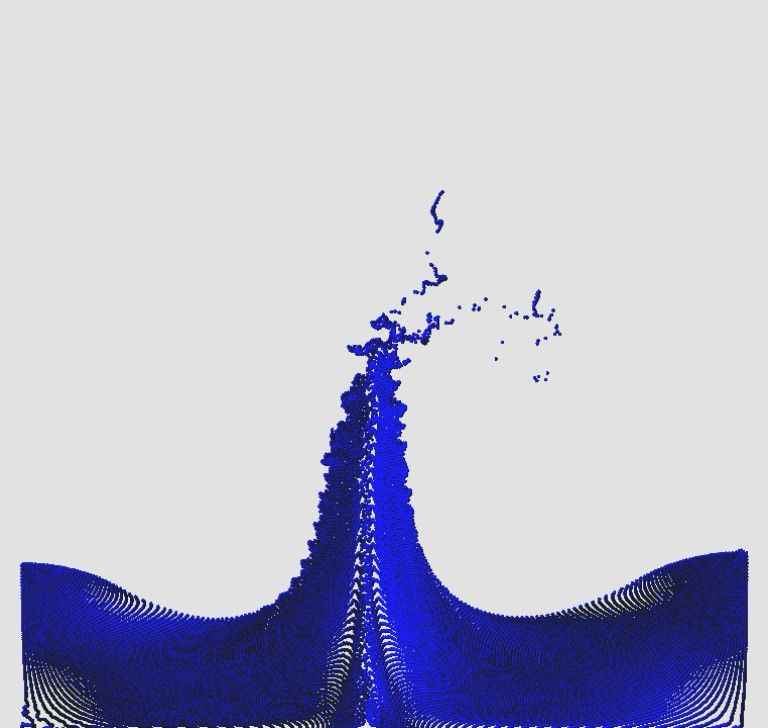
\includegraphics[width=\textwidth]{DDB/DDB-05.jpg}
	\end{subfigure}
	\begin{subfigure}[!h]{0.3\textwidth} \centering
		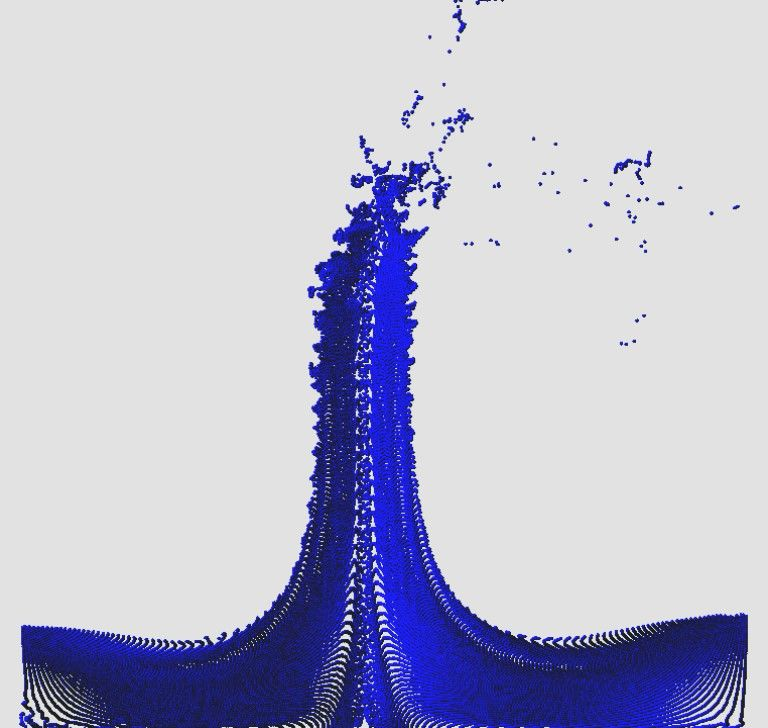
\includegraphics[width=\textwidth]{DDB/DDB-06.jpg}
	\end{subfigure}
	\begin{subfigure}[!h]{0.3\textwidth} \centering
		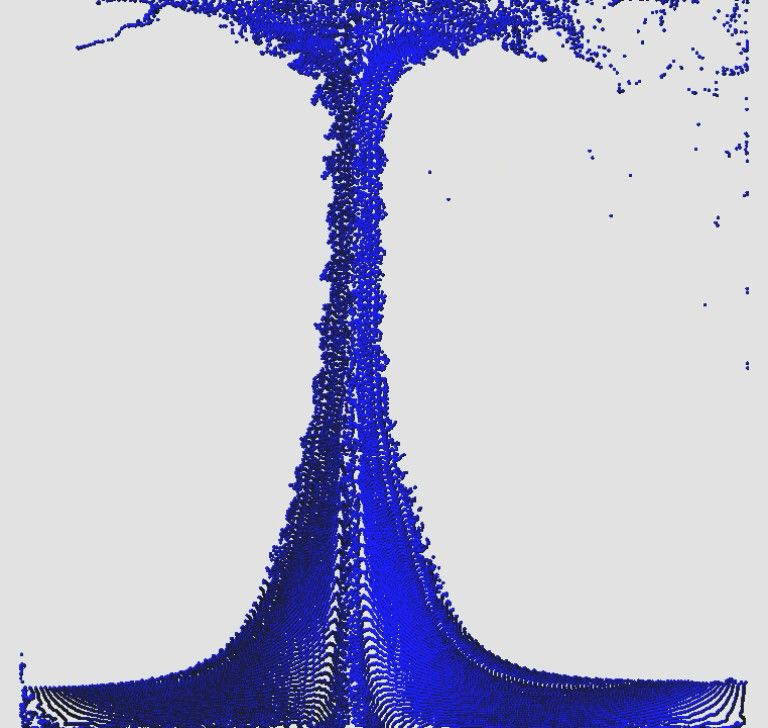
\includegraphics[width=\textwidth]{DDB/DDB-07.jpg}
	\end{subfigure}
	\begin{subfigure}[!h]{0.3\textwidth} \centering
		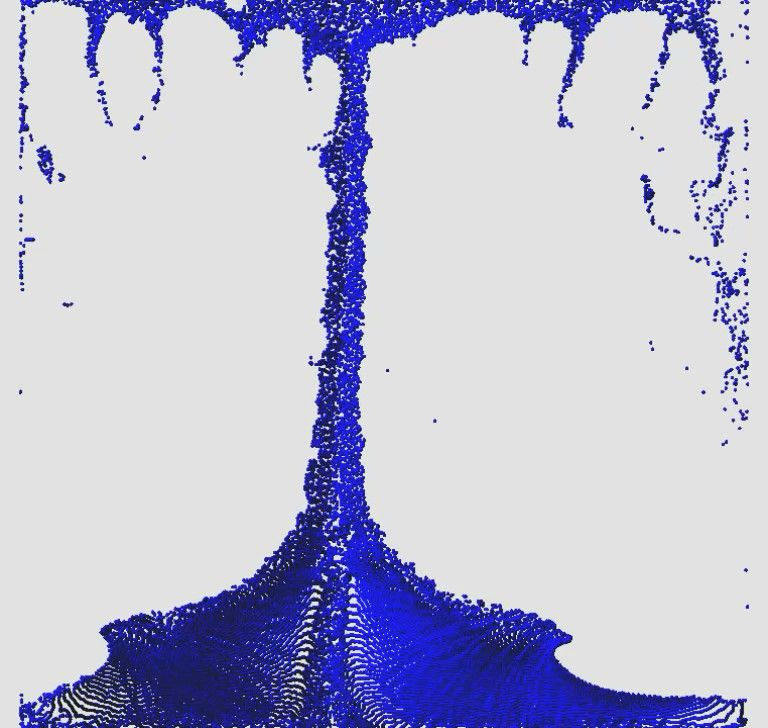
\includegraphics[width=\textwidth]{DDB/DDB-08.jpg}
	\end{subfigure}
	\begin{subfigure}[!h]{0.3\textwidth} \centering
		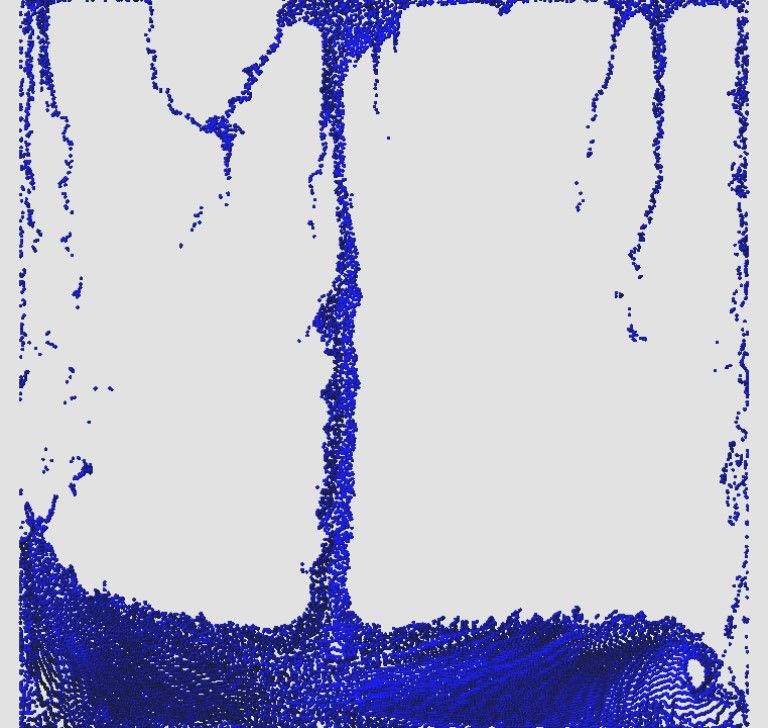
\includegraphics[width=\textwidth]{DDB/DDB-09.jpg}
	\end{subfigure}
	\begin{subfigure}[!h]{0.3\textwidth} \centering
		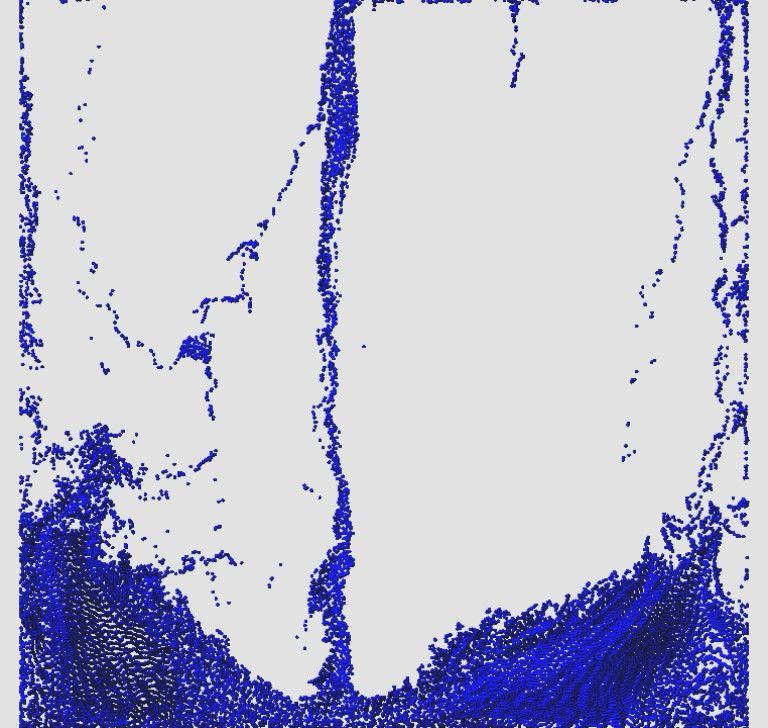
\includegraphics[width=\textwidth]{DDB/DDB-10.jpg}
	\end{subfigure}
	\begin{subfigure}[!h]{0.3\textwidth} \centering
		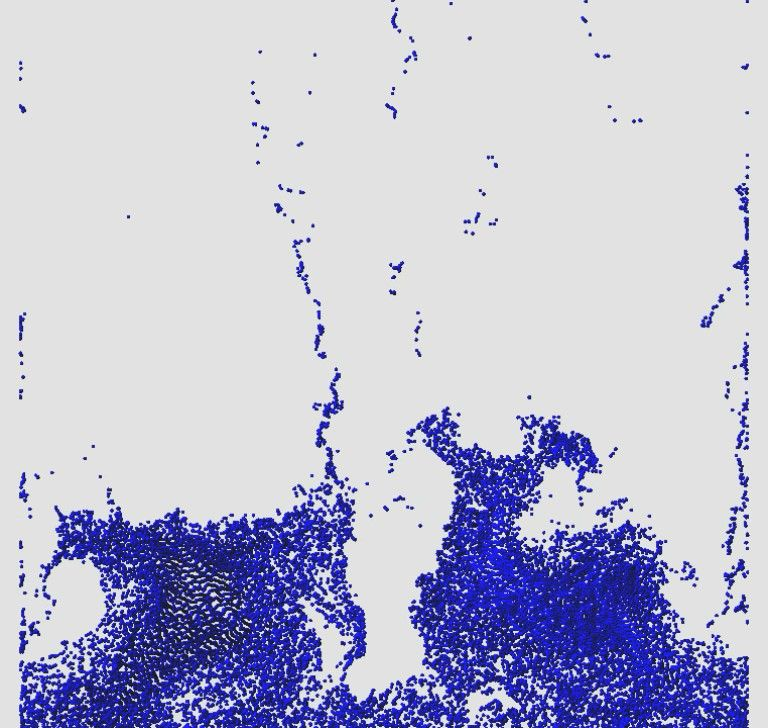
\includegraphics[width=\textwidth]{DDB/DDB-11.jpg}
	\end{subfigure}
    \caption{Simulação \textit{Double Dam Breaking} de um fluido invíscido.}
    \label{fig:doubledb}
\end{figure}

\begin{figure}[!h] \centering
	\begin{subfigure}[!h]{0.3\textwidth} \centering
		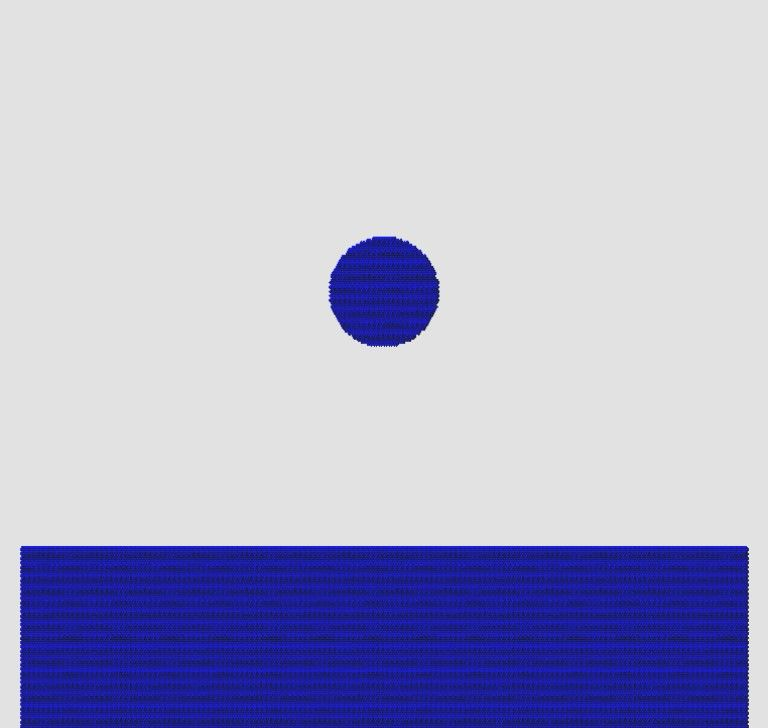
\includegraphics[width=\textwidth]{WD/WD-01.jpg}
	\end{subfigure}
    \begin{subfigure}[!h]{0.3\textwidth} \centering
		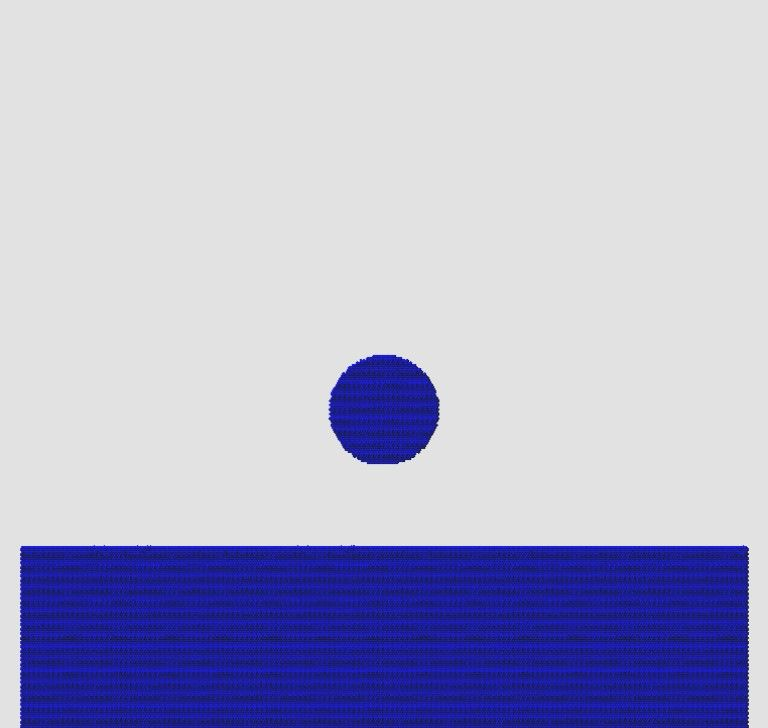
\includegraphics[width=\textwidth]{WD/WD-02.jpg}
	\end{subfigure}
	\begin{subfigure}[!h]{0.3\textwidth} \centering
		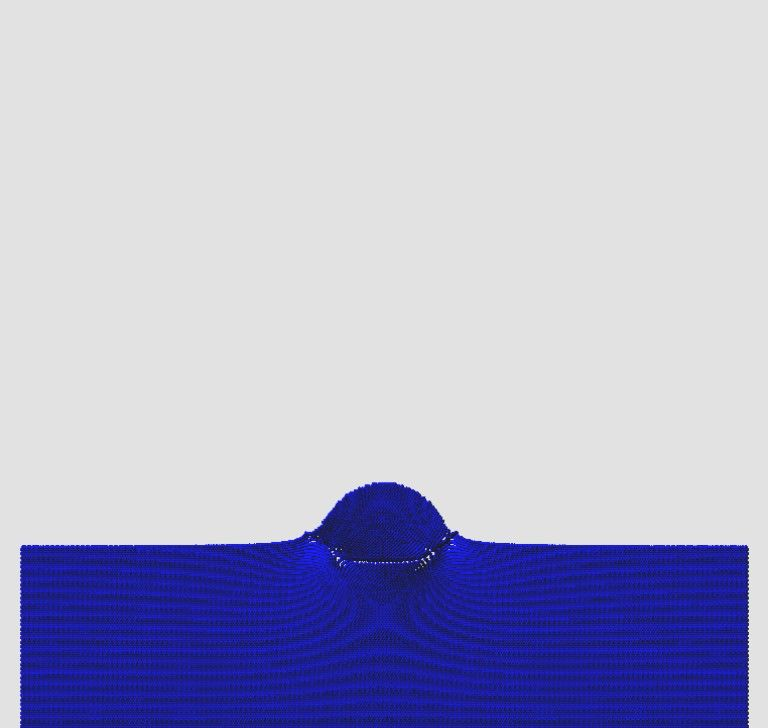
\includegraphics[width=\textwidth]{WD/WD-03.jpg}
	\end{subfigure}
	\begin{subfigure}[!h]{0.3\textwidth} \centering
		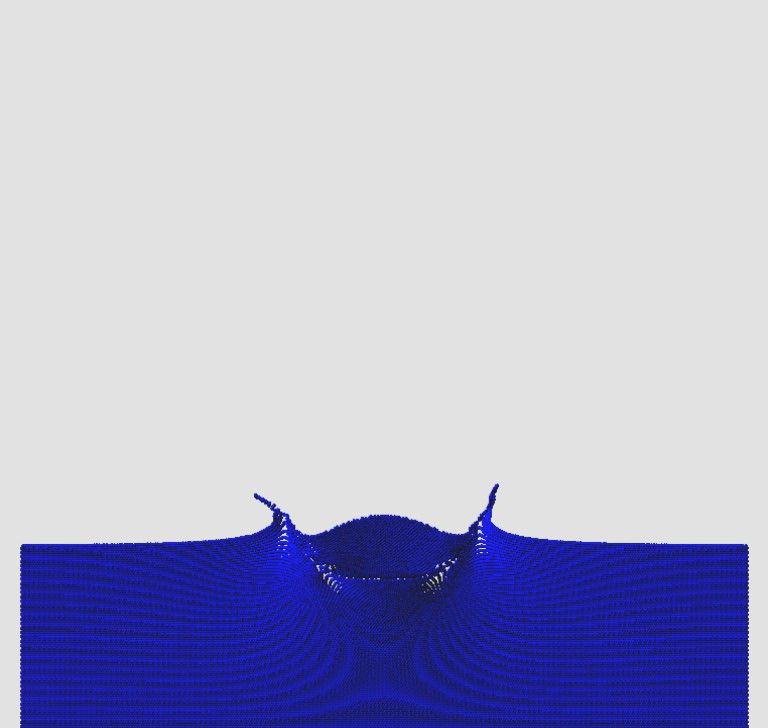
\includegraphics[width=\textwidth]{WD/WD-04.jpg}
	\end{subfigure}
	\begin{subfigure}[!h]{0.3\textwidth} \centering
		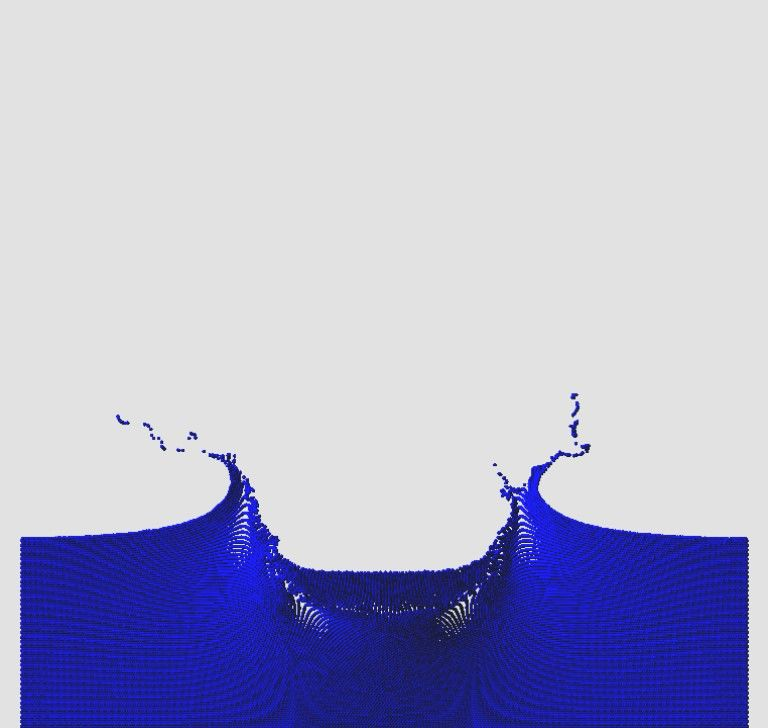
\includegraphics[width=\textwidth]{WD/WD-05.jpg}
	\end{subfigure}
	\begin{subfigure}[!h]{0.3\textwidth} \centering
		\includegraphics[width=\textwidth]{WD/WD-06.jpg}
	\end{subfigure}
	\begin{subfigure}[!h]{0.3\textwidth} \centering
		\includegraphics[width=\textwidth]{WD/WD-07.jpg}
	\end{subfigure}
	\begin{subfigure}[!h]{0.3\textwidth} \centering
		\includegraphics[width=\textwidth]{WD/WD-08.jpg}
	\end{subfigure}
	\begin{subfigure}[!h]{0.3\textwidth} \centering
		\includegraphics[width=\textwidth]{WD/WD-09.jpg}
	\end{subfigure}
	\begin{subfigure}[!h]{0.3\textwidth} \centering
		\includegraphics[width=\textwidth]{WD/WD-10.jpg}
	\end{subfigure}
	\begin{subfigure}[!h]{0.3\textwidth} \centering
		\includegraphics[width=\textwidth]{WD/WD-11.jpg}
	\end{subfigure}
	\begin{subfigure}[!h]{0.3\textwidth} \centering
		\includegraphics[width=\textwidth]{WD/WD-12.jpg}
	\end{subfigure}
    \caption{Simulação \textit{Water Drop} de um fluido invíscido.}
    \label{fig:waterdrop}
\end{figure}

\clearpage

% [TODO] explicar que foi feita uma avaliação qualitativa
% Este tipo de avaliação foi adotado pois uma avaliação quantitativa dos resultados implicaria no uso de métricas que permitissem verificar diferenças com outros resultados da literatura, como por exemplo avaliar a diferença das posições e velocidades das partículas.A avaliação das simulações obtidas na execução do código é qualitativa, ou seja, avaliada visualmente em comparação com os resultados de

\section{Conclusão}
\label{sec:conclusion}

Neste trabalho de conclusão de curso estudaram-se métodos híbridos, especificamente os que utilizam partículas e grade regular, para a simulação de fluidos viscosos incompressíveis em duas dimensões. O uso da grade regular implica no uso de métodos numéricos para a resolução de operadores diferenciais presentes nas equações de modelam os fluidos incompressíveis, o método mais comum sendo o das diferenças finitas. Além do estudo destes métodos, foi proposta uma implementação orientada a objetos do método híbrido FLIP, que estende o método PIC em busca de menor dissipação numérica.

De acordo com o proposto para este trabalho, os objetivos específicos foram alcançados na totalidade, vistos os resultados apresentados. Dentre as dificuldades enfrentadas no desenvolvimento deste trabalho, destacam-se as relacionadas ao entendimento da parte teórica que precede a implementação, e também as provenientes da implementação dos diversos componentes do sistema, que devem estar em perfeita sincronia para a execução apropriada.

Visto que o código desenvolvido é capaz de simular fluidos para duas dimensões, futuramente pretende-se estender a implementação para o caso tridimensional. Além disso, uma melhoria possível é o uso de programação paralela, tanto em CPU quanto em GPU, para acelerar a execução da simulação. Por fim, este trabalho servirá de base para um projeto de mestrado que propõe o uso de grades adaptativas como alternativa às grades regulares, usadas neste trabalho. Grades adaptativas são subdividem o espaço em árvores quaternária e octária nos casos bidimensionais e tridimensionais, respectivamente. 

\footnotesize
\bibliography{tcc}
\bibliographystyle{acm}

\end{document}
